\subsection{Analytic 2x2}


\subsubsection{Microstates 2x2}

\begin{center}
\label{tab:states-2x2}
\captionof{table}{This shows the different microstates that is possible for a 2x2 spinmatrix. It also states the energy and magnetic moment for each microstate.}
\begin{tabularx}{\textwidth}{c c c X c c c}
    \hline 
    \hline 
        State & Energy & Magnetic moment && State & Energy & Magnetic moment \\ 
    \hline
        \tilstand{1}{1}{1}{1} & -8J & 4 && \tilstand{0}{0}{0}{0} & -8J & -4 \\ \\
        
        \tilstand{0}{1}{1}{1} & 0J & 2 && \tilstand{1}{0}{0}{0} & 0J & -2 \\ \\
        \tilstand{1}{0}{1}{1} & 0J & 2 && \tilstand{0}{1}{0}{0} & 0J & -2 \\ \\
        \tilstand{1}{1}{0}{1} & 0J & 2 && \tilstand{0}{0}{1}{0} & 0J & -2 \\ \\
        \tilstand{1}{1}{1}{0} & 0J & 2 && \tilstand{0}{0}{0}{1} & 0J & -2 \\ \\

        \tilstand{0}{0}{1}{1} & 0J & 0 && \tilstand{1}{1}{0}{0} & 0J & 0 \\ \\ 
        \tilstand{0}{1}{0}{1} & 0J & 0 && \tilstand{1}{0}{1}{0} & 0J & 0 \\ \\
        \tilstand{1}{0}{0}{1} & 8J & 0 && \tilstand{0}{1}{1}{0} & 8J & 0 \\ \\
    \hline
\end{tabularx}
\end{center}



\begin{center}
\label{tab:states-2x2-summary}
\captionof{table}{The table shows a summary from table \ref{tab:states-2x2}. }
\begin{tabularx}{\textwidth}{c X c X c X c}
    \hline 
    \hline 
        Number of $\color{red}{\uparrow}$ && Multiplicity && Energy && Magnetic moment \\ 
    \hline
        4   &&      1      &&      -8J     &&       4       \\  
        3   &&      4      &&      0J      &&       2       \\
        2   &&      2      &&      8J      &&       0       \\
        2   &&      4      &&      0J      &&       0       \\
        1   &&      4      &&      0J      &&       -2      \\
        0   &&      1      &&      -8J     &&       -4      \\
    \hline
\end{tabularx}
\end{center}












\pagebreak
\subsubsection{Quantities}

We will use the equations from section \ref{sec:expect}.
\\
\\
For energy the eq. \ref{eq:E} will result in:

\begin{align*}
    &Z = \sum_i = e^{-\beta E_i}
    \\
    &\text{T = kT/J = 1} 
    \\
    &Z = \sum_i = e^{-\beta E_i} = 2e^{8} + 2e^{-8} + 12
\end{align*}


For energy the eq. \ref{eq:E} will give the result:

\begin{align*}
    &\langle E \rangle = \sum_i E_iP(E_i)
    \\
    &\text{T = kT/J = 1} 
    \\
    &\langle E \rangle = \frac{1}{Z} \sum_i E_i e^{-E_i}
    \\
    &\langle E \rangle = \frac{1}{Z} \left( -16 e^8 + 16e^{-8} \right) = -7.9839
    \\ 
    &\langle E \rangle /N= \frac{\langle E \rangle}{4} = -1.9959
\end{align*}


For energy the eq. \ref{eq:M} will give the result:

\begin{align*}
    &\langle |M| \rangle = \sum_i M_iP(E_i)
    \\
    &\text{T = kT/J = 1} 
    \\
    &\langle |M| \rangle = \frac{1}{Z} \sum_i M_i e^{-E_i}
    \\
    &\langle |M| \rangle 
    = 
    \frac{1}{Z} 
    \left(
      4\cdot1e^{8} 
    + 2\cdot4e^{0} 
    + 0\cdot2e^{-8} 
    + 0\cdot4e^{0} 
    + 2\cdot4e^{0}  
    + 4\cdot1e^{8}
    \right) 
    \\
    &\langle |M| \rangle 
    = 
    \frac{1}{Z} 
    \left(
    16
    + 8 e^{8}
    \right) = 3.9946
    \\ 
    &\langle |M| \rangle /N= \frac{\langle M \rangle}{4} = 0.9986
\end{align*}


\pagebreak
For $C_V$ we need to calculate $\langle E^2 \rangle$:

\begin{align*}
    &\langle E^2 \rangle = \sum_i E_iP(E_i)
    \\
    &\text{T = kT/J = 1} 
    \\
    &\langle E^2 \rangle = \frac{1}{Z} \sum_i E_i^2 e^{-E_i}
    \\
    &\langle E^2 \rangle = \frac{1}{Z} \left( 128 e^8 + 128 e^{-8} \right)
    \\
    &C_V = \langle E^2 \rangle - \langle E \rangle^2 = 0.12832
    \\ 
    &C_V/N = 0.03208
\end{align*}



For $\chi$ we need to calculate $\langle M^2 \rangle$:

\begin{align*}
    &\langle M^2 \rangle = \sum_i M_i^2P(E_i)
    \\
    &\text{T = kT/J = 1} 
    \\
    &\langle M^2 \rangle = \frac{1}{Z} \sum_i M_i^2 e^{-E_i}
    \\
    &\langle M^2 \rangle 
    = 
    \frac{1}{Z} 
    \left(
      16\cdot1e^{8} 
    + 4\cdot4e^{0} 
    + 0\cdot2e^{-8} 
    + 0\cdot4e^{0} 
    + 4\cdot4e^{0}  
    + 16\cdot1e^{8}
    \right) 
    \\
    &\langle M^2 \rangle 
    = 
    \frac{1}{Z} 
    \left(
    32
    + 32 e^{8}
    \right) = 15.9732
    \\
    &\langle \chi \rangle = 0.01604
    \\
    &\langle \chi \rangle / N = 0.004010
\end{align*}

Below you can see a summary for the quantities:

\begin{align*}
    \langle E \rangle /N &= -1.9959  \qquad &&\langle |M| \rangle /N = 0.9986
    \\
    C_V/N &= 0.03208  \qquad &&\langle \chi \rangle / N = 0.004010
\end{align*}
























\pagebreak
\subsection{Simulation 2x2}

These simulations ran for $10^5$ Monte Carlo cycles. All the simulations were done at T=1 and for a 2x2 grid. In general the left sub figure is the actual value plotted with the analytic answer and the right sub figure is the difference for analytic and simulated value.
All the values converges at about 40\% of the Monte Carlo cycles.

\begin{figure}[H]
    \centering
    \begin{subfigure}{0.5\textwidth}
        \centering
        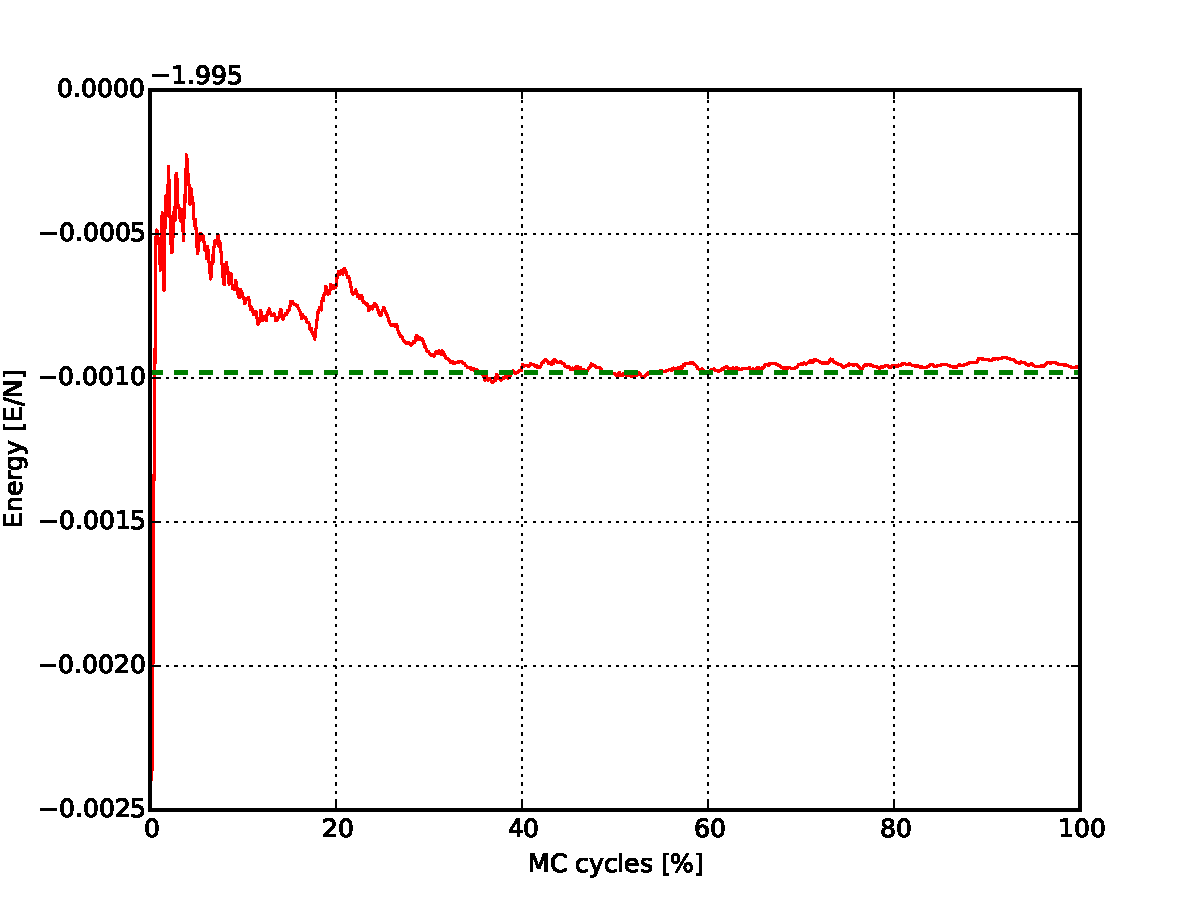
\includegraphics[width=\linewidth]{result/bilder/2x2/energy22}
        \caption{}
    \end{subfigure}%
    ~ 
    \begin{subfigure}{0.5\textwidth}
        \centering
        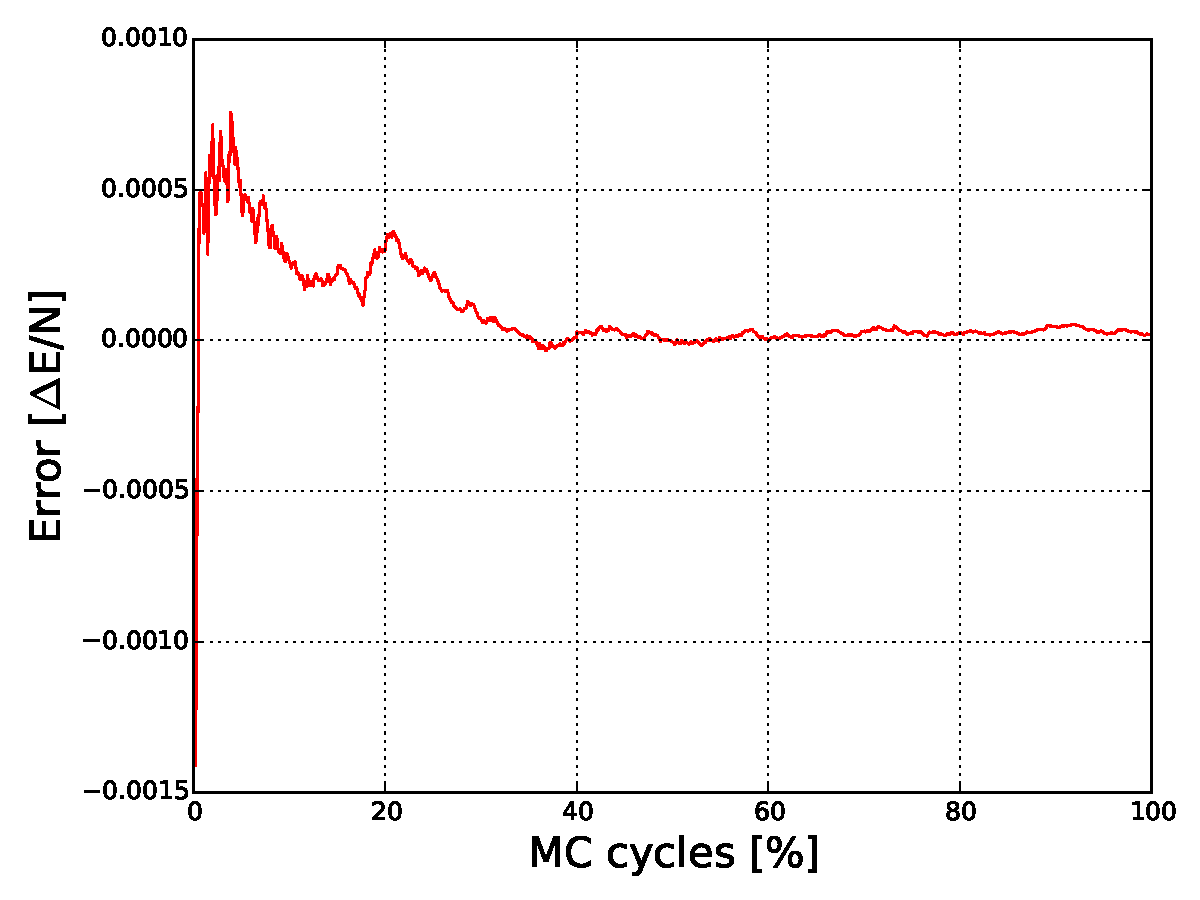
\includegraphics[width=\linewidth]{result/bilder/2x2/energyerror22}
        \caption{}
    \end{subfigure}
    \caption{a) Shows how the expectation value for E varies versus Monte Carlo cycles. b) Shows how the error develops.}
    \label{fig:22-energy}
\end{figure}

\begin{figure}[H]
    \centering
    \begin{subfigure}{0.5\textwidth}
        \centering
        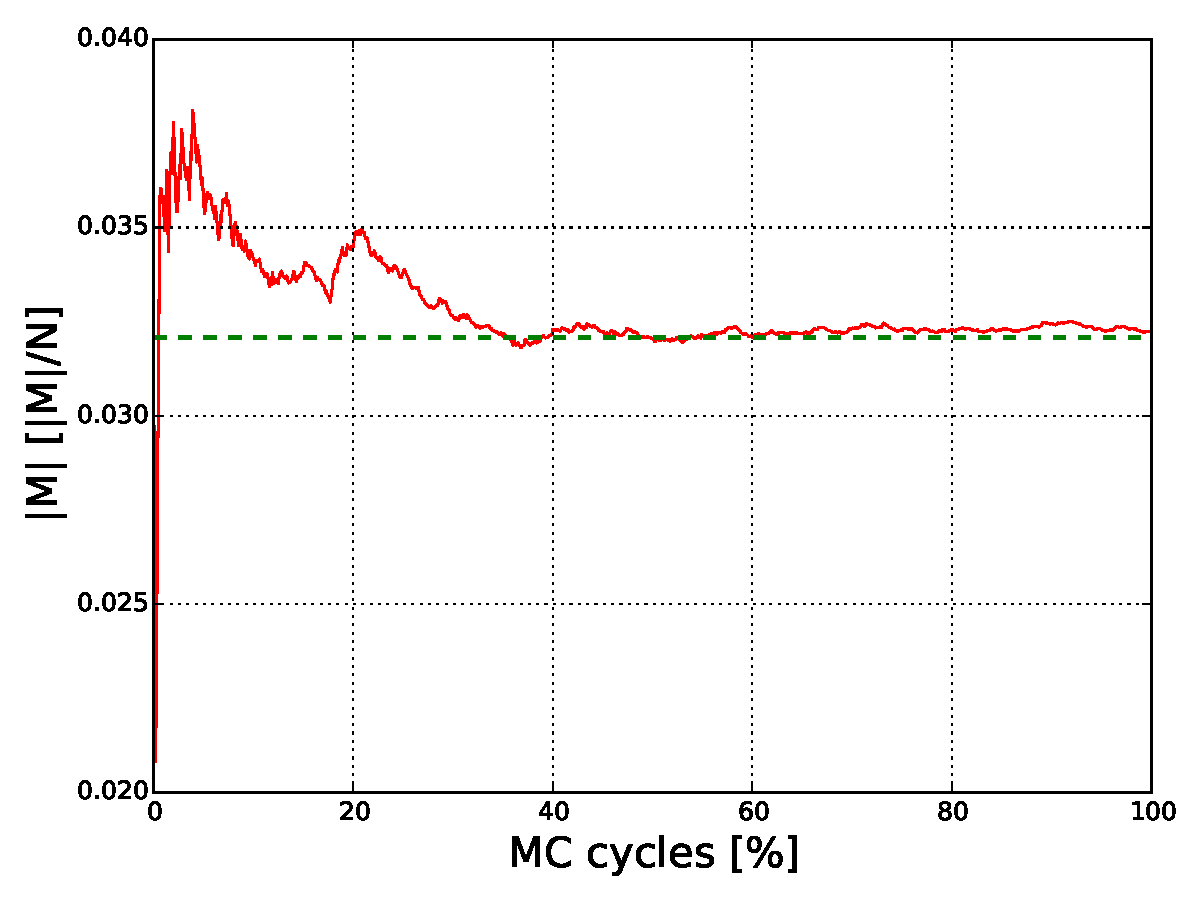
\includegraphics[width=\linewidth]{result/bilder/2x2/cv22}
        \caption{}
    \end{subfigure}%
    ~ 
    \begin{subfigure}{0.5\textwidth}
        \centering
        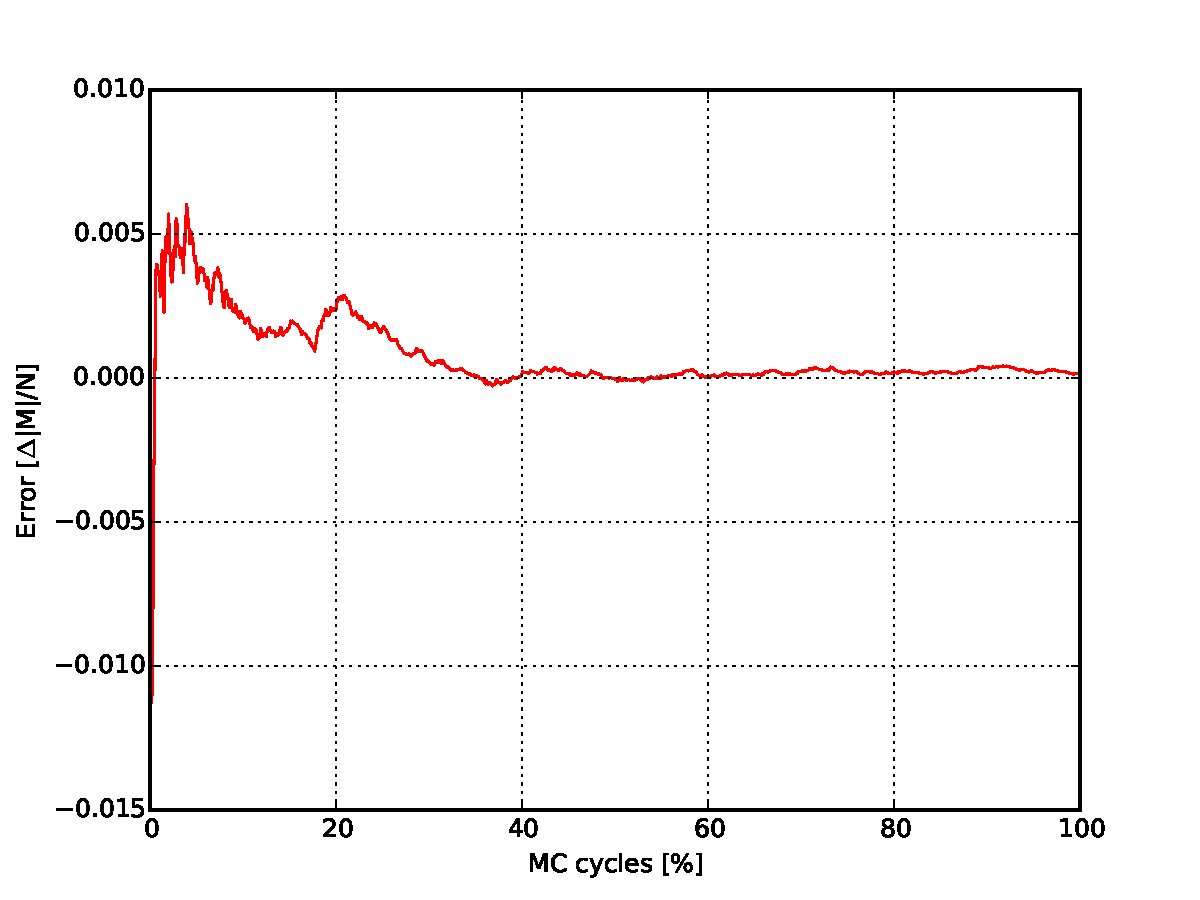
\includegraphics[width=\linewidth]{result/bilder/2x2/cverror22}
        \caption{}
    \end{subfigure}
    \caption{a) Shows how the expectation value for $C_V$ varies versus Monte Carlo cycles. b) Shows how the error develops. }
    \label{fig:22-cv}
\end{figure}

\begin{figure}[H]
    \centering
    \begin{subfigure}{0.5\textwidth}
        \centering
        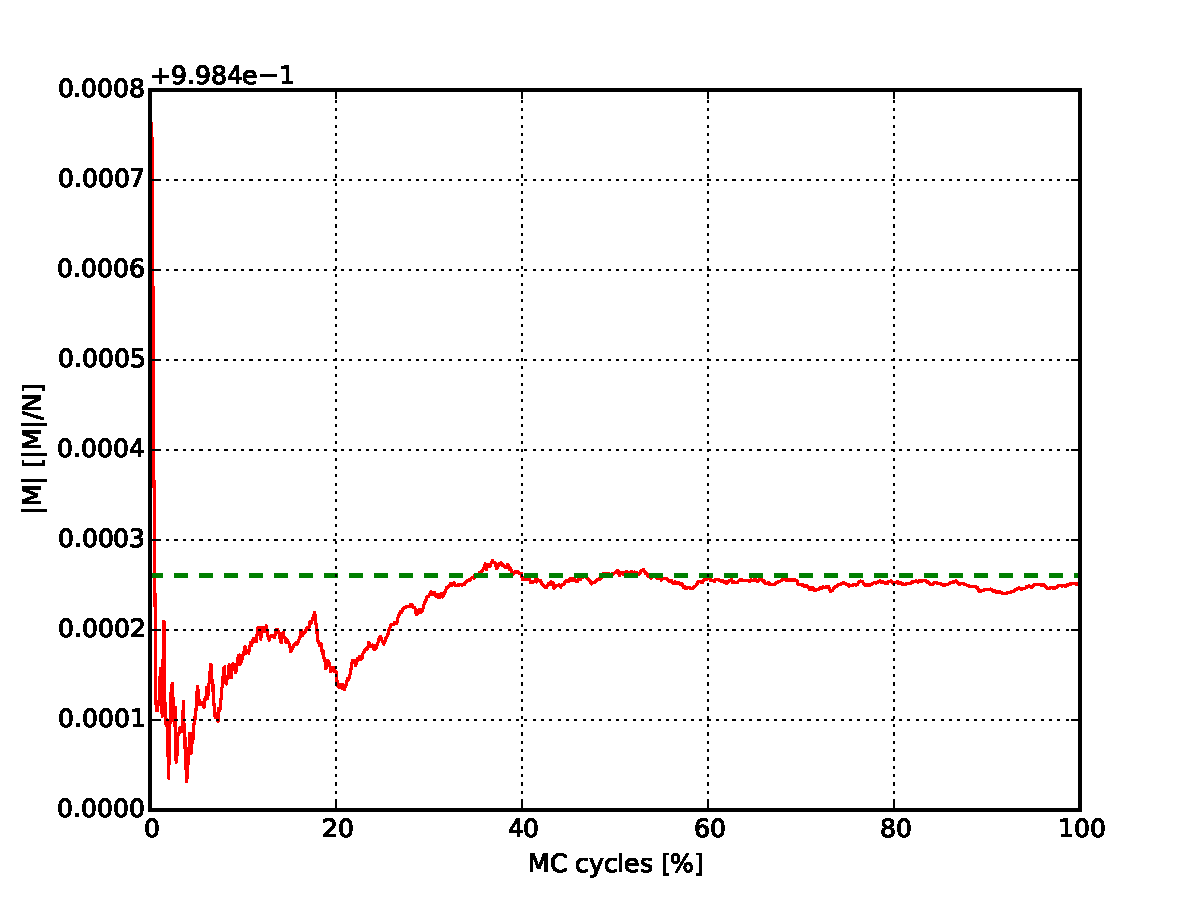
\includegraphics[width=\linewidth]{result/bilder/2x2/mabs22}
        \caption{}
    \end{subfigure}%
    ~ 
    \begin{subfigure}{0.5\textwidth}
        \centering
        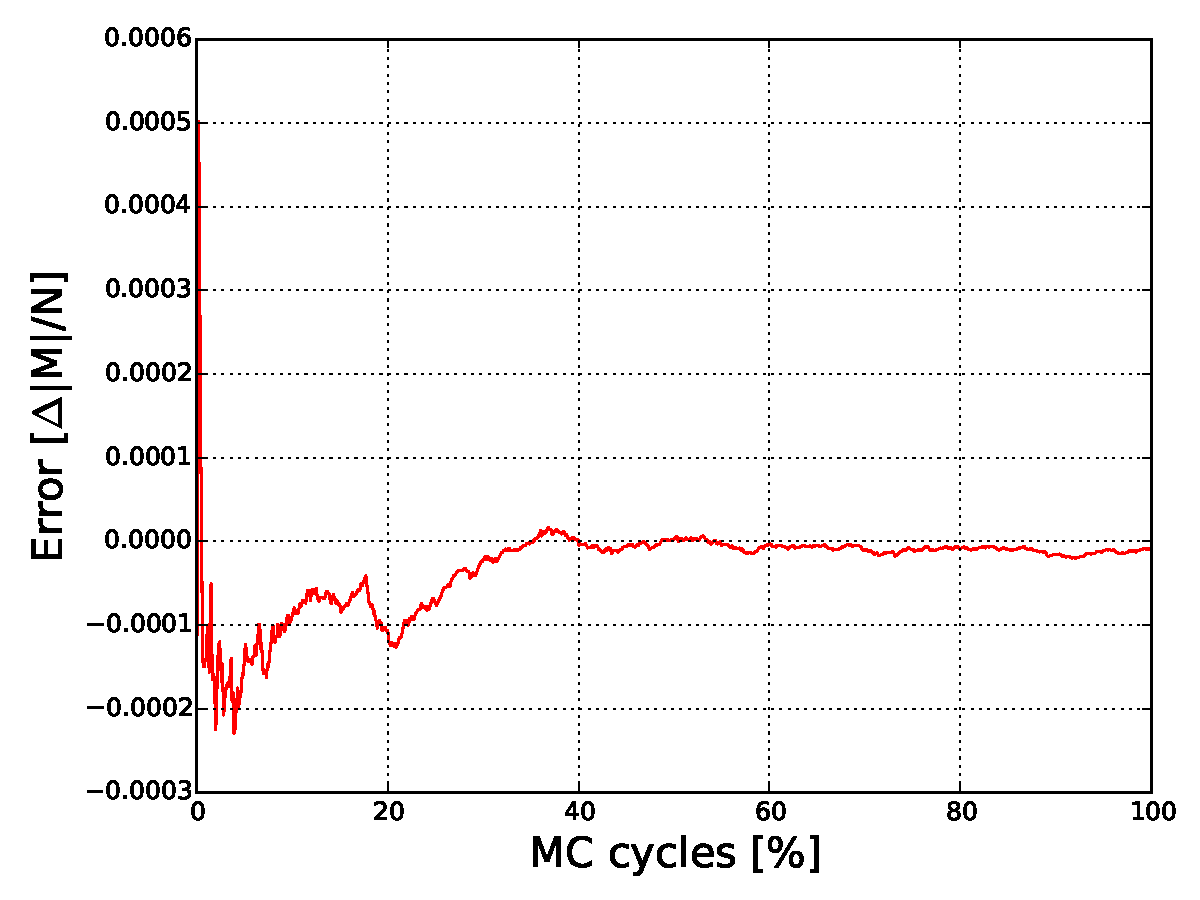
\includegraphics[width=\linewidth]{result/bilder/2x2/mabserror22}
        \caption{}
    \end{subfigure}
    \caption{a) Shows how the expectation value for |M| varies versus Monte Carlo cycles. b) Shows how the error develops.}
    \label{fig:22-m}
\end{figure}

\begin{figure}[H]
    \centering
    \begin{subfigure}{0.5\textwidth}
        \centering
        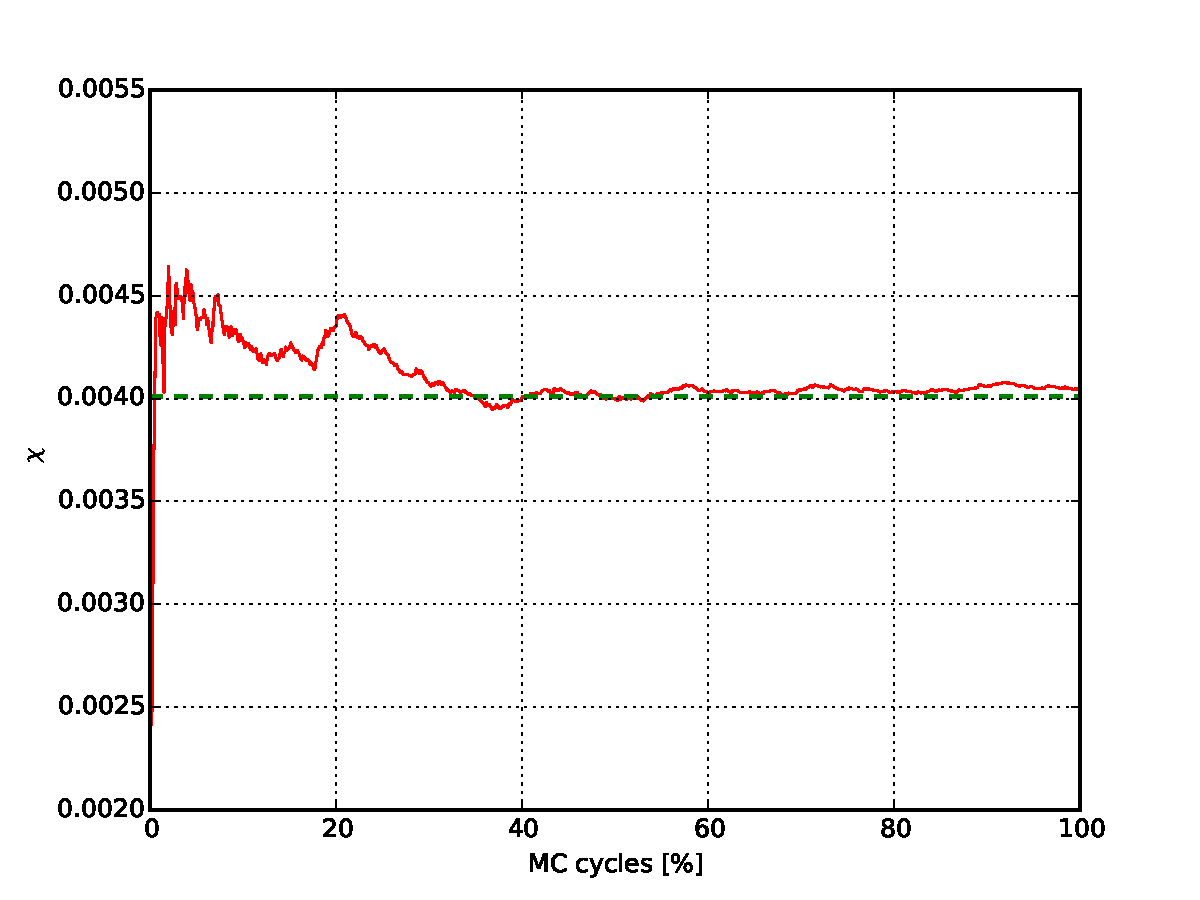
\includegraphics[width=\linewidth]{result/bilder/2x2/chi22}
        \caption{}
    \end{subfigure}%
    ~ 
    \begin{subfigure}{0.5\textwidth}
        \centering
        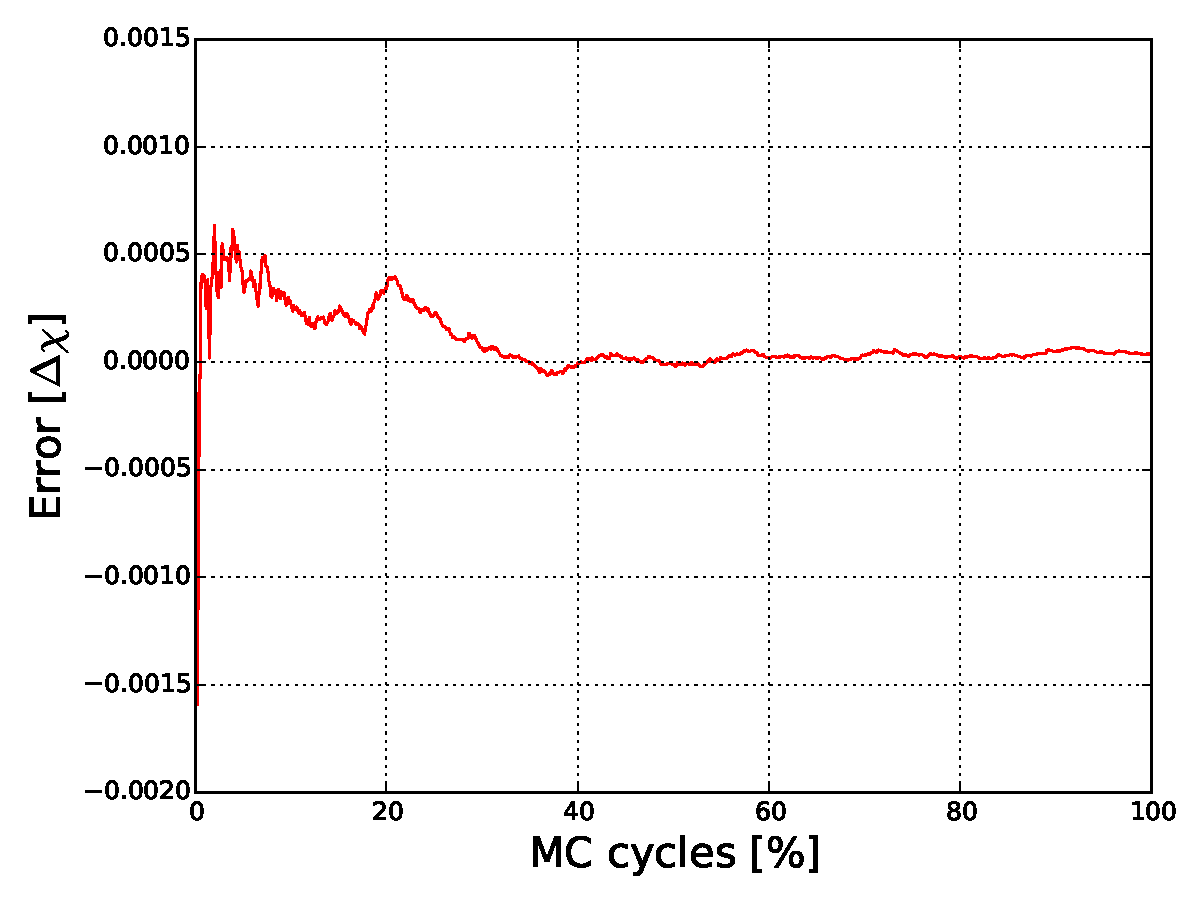
\includegraphics[width=\linewidth]{result/bilder/2x2/chierror22}
        \caption{}
    \end{subfigure}
    \caption{a) Shows how the expectation value for $\chi$ varies versus Monte Carlo cycles. b) Shows how the error develops.}
    \label{fig:22-chi}
\end{figure}


















\pagebreak
\subsection{Convergence of 20x20}

In this section convergence for a 20x20 grid is studied. All grids were simulated for 10 million Monte Carlo cycles. Unless something else is specified in the figure, the left figure is for a initial configuration of the spin in the same direction and the right figure is for a random configuration. 

\begin{figure}[H]
    \centering
    \begin{subfigure}{0.5\textwidth}
        \centering
        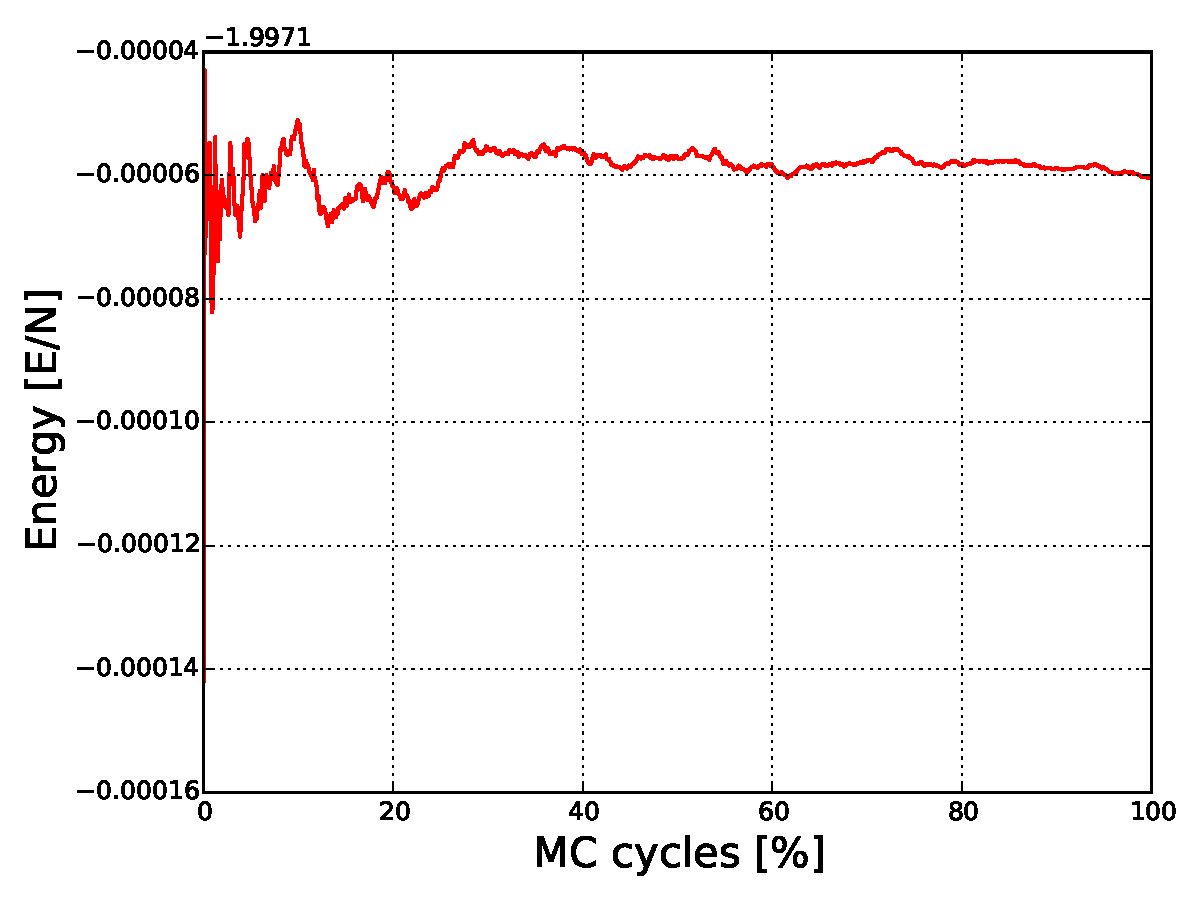
\includegraphics[width=\linewidth]{result/bilder/20x20/E-N20-T1}
        \caption{}
    \end{subfigure}%
    ~ 
    \begin{subfigure}{0.5\textwidth}
        \centering
        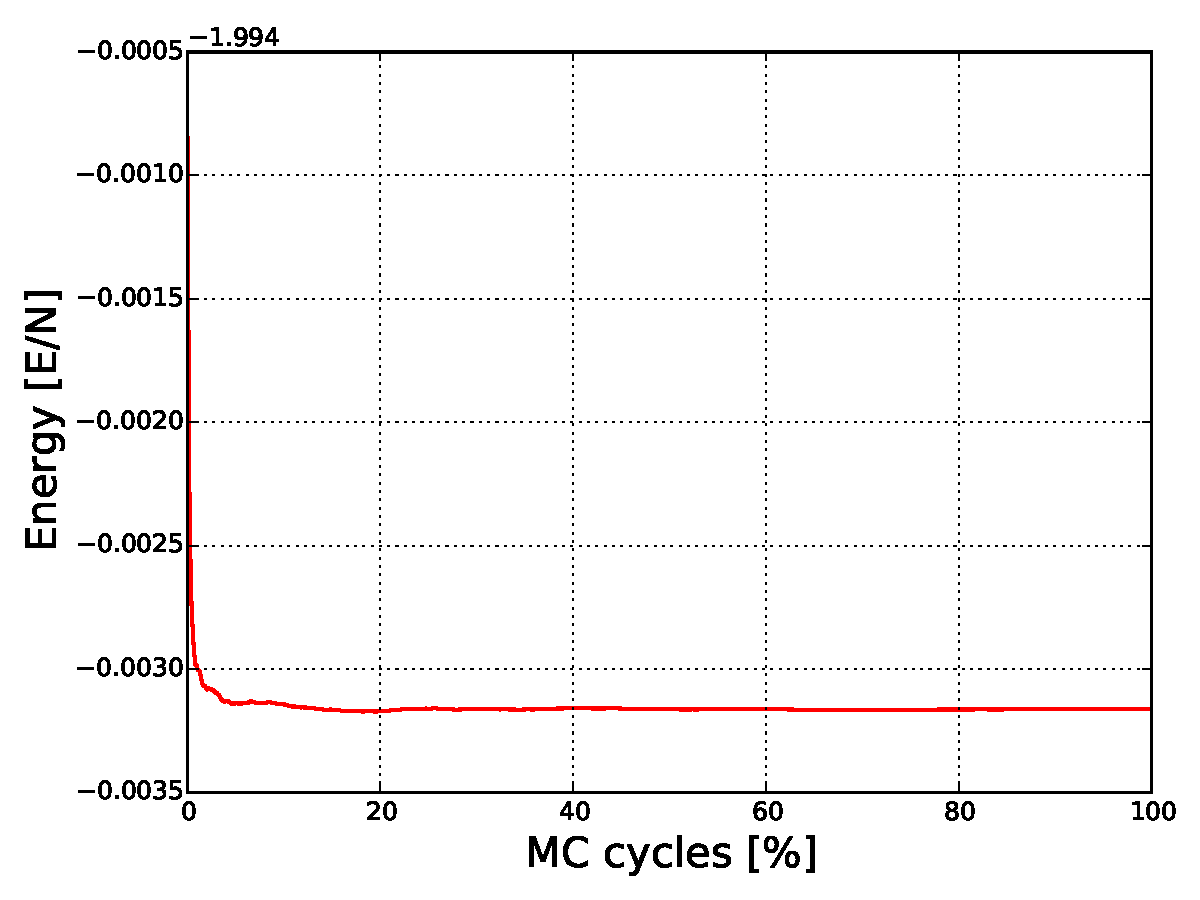
\includegraphics[width=\linewidth]{result/bilder/20x20/E-N20-T1-RNG}
        \caption{}
    \end{subfigure}
    \caption{The figure shows the development of E when T = 1. }
    \label{fig:}
\end{figure}

\begin{figure}[H]
    \centering
    \begin{subfigure}{0.5\textwidth}
        \centering
        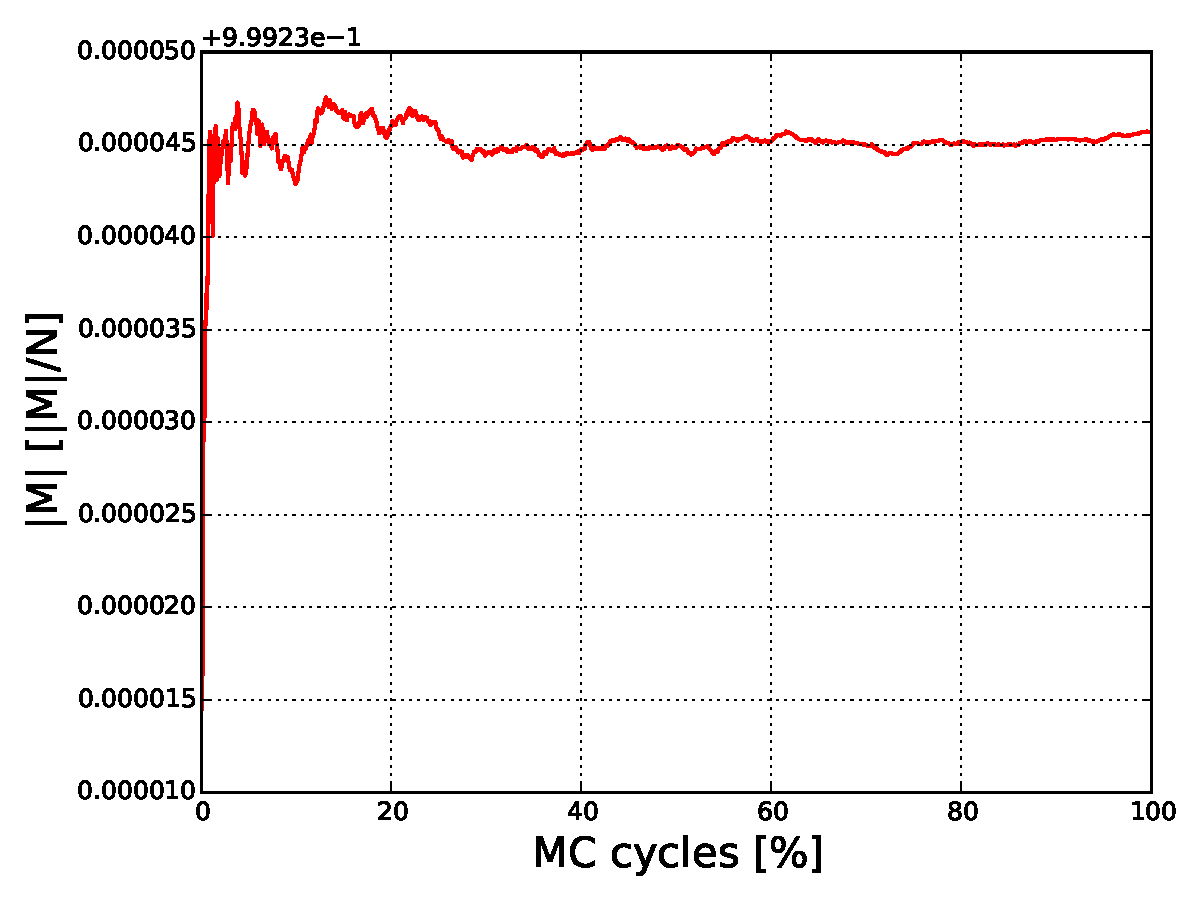
\includegraphics[width=\linewidth]{result/bilder/20x20/M-N20-T1}
        \caption{}
    \end{subfigure}%
    ~ 
    \begin{subfigure}{0.5\textwidth}
        \centering
        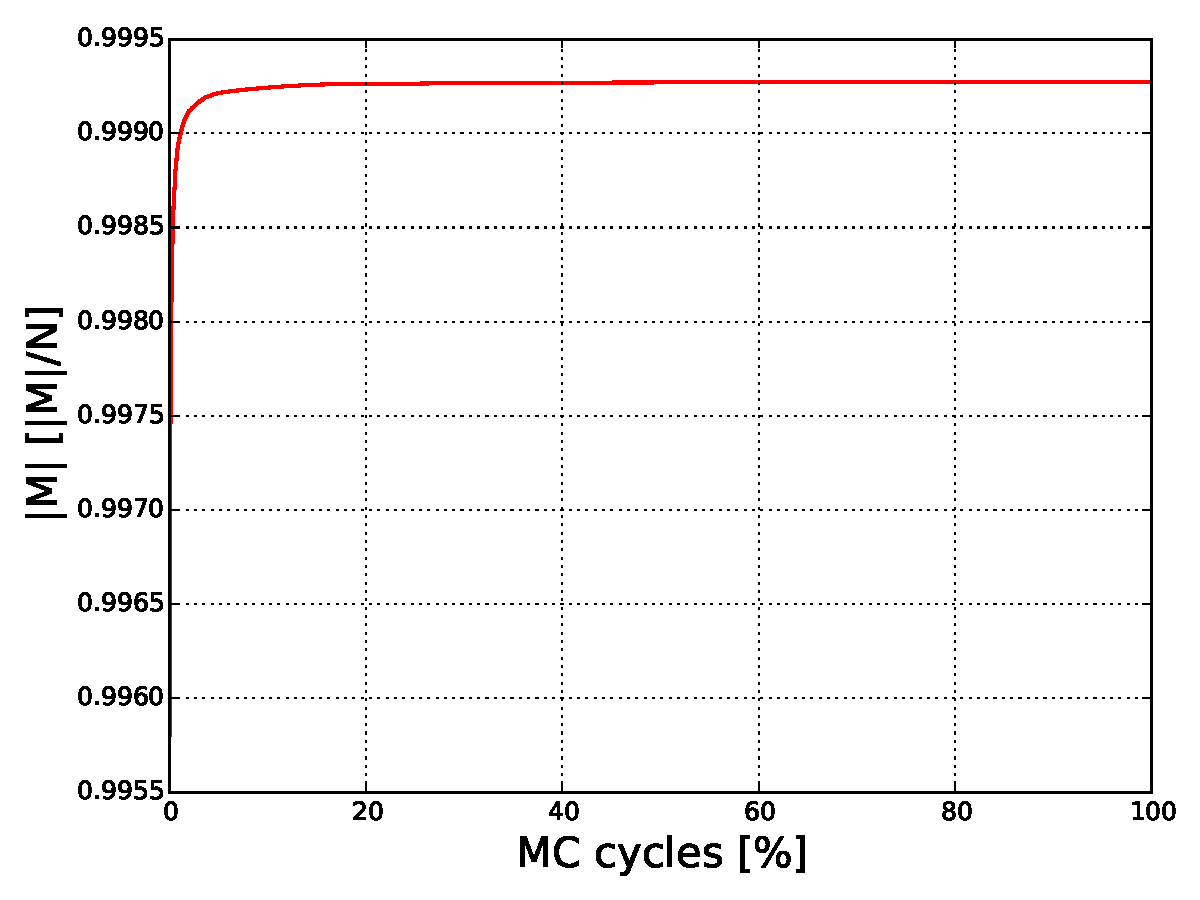
\includegraphics[width=\linewidth]{result/bilder/20x20/M-N20-T1-RNG}
        \caption{}
    \end{subfigure}
    \caption{The figure shows the development of |M| when T = 1. }
    \label{fig:}
\end{figure}






\begin{figure}[H]
    \centering
    \begin{subfigure}{0.5\textwidth}
        \centering
        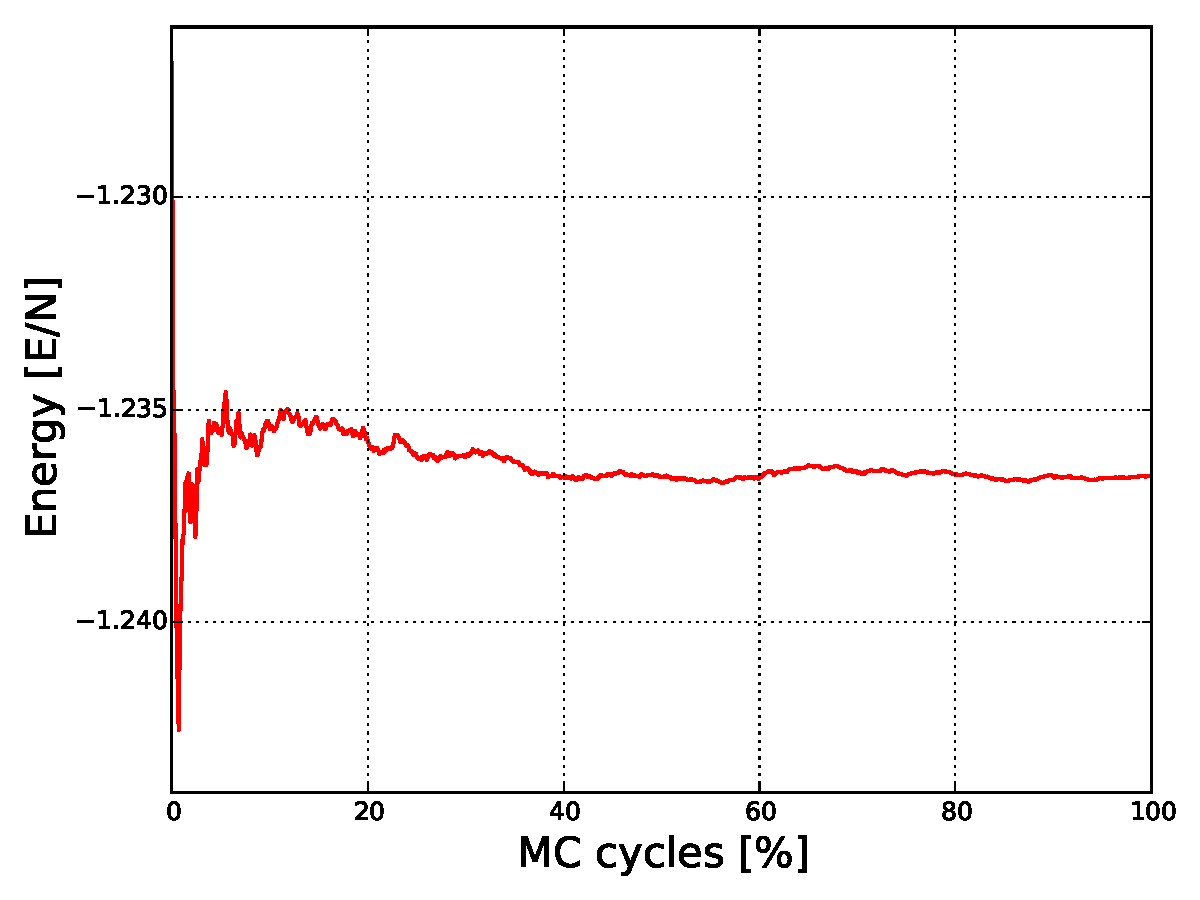
\includegraphics[width=\linewidth]{result/bilder/20x20/E-N20-T24}
        \caption{}
    \end{subfigure}%
    ~ 
    \begin{subfigure}{0.5\textwidth}
        \centering
        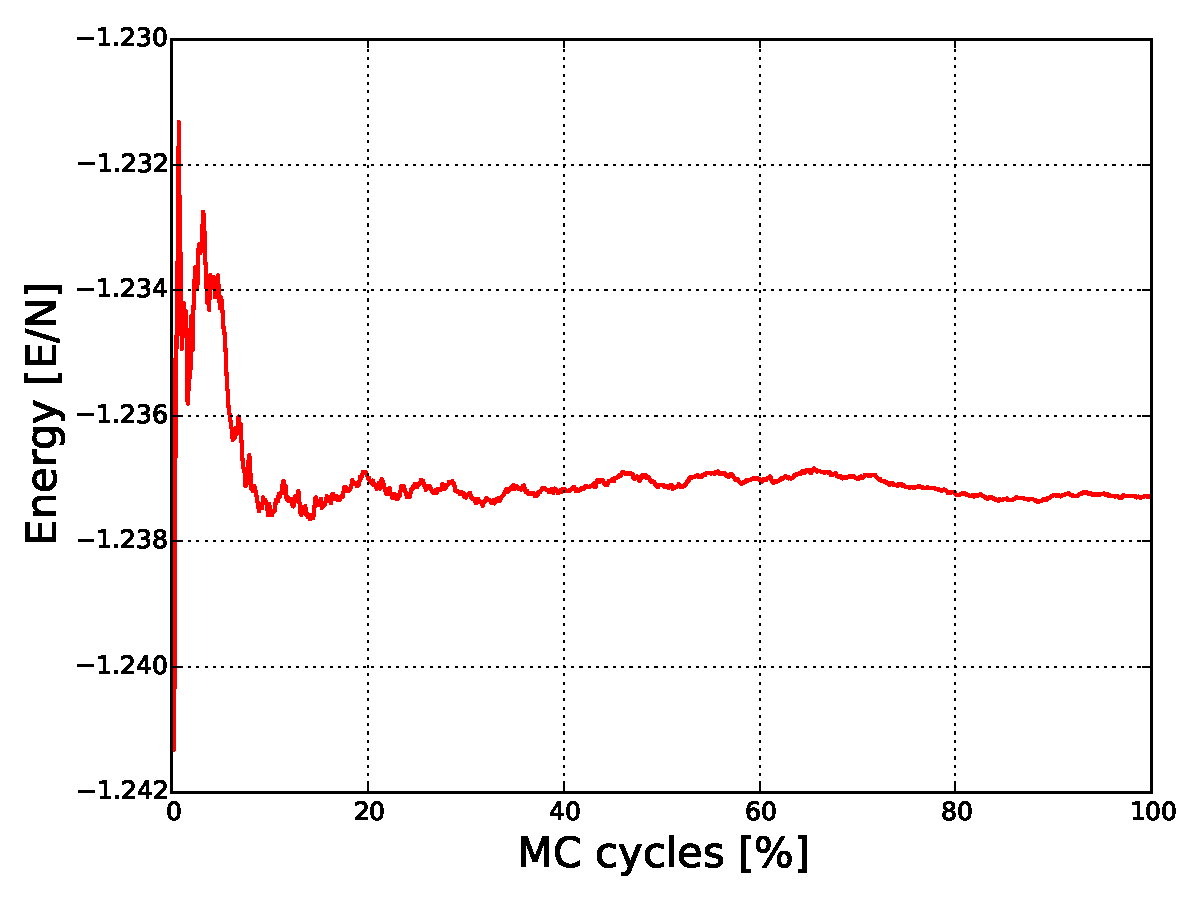
\includegraphics[width=\linewidth]{result/bilder/20x20/E-N20-T24-RNG}
        \caption{}
    \end{subfigure}
    \caption{The figure shows the development of E when T = 2.4 . }
    \label{fig:}
\end{figure}

\begin{figure}[H]
    \centering
    \begin{subfigure}{0.5\textwidth}
        \centering
        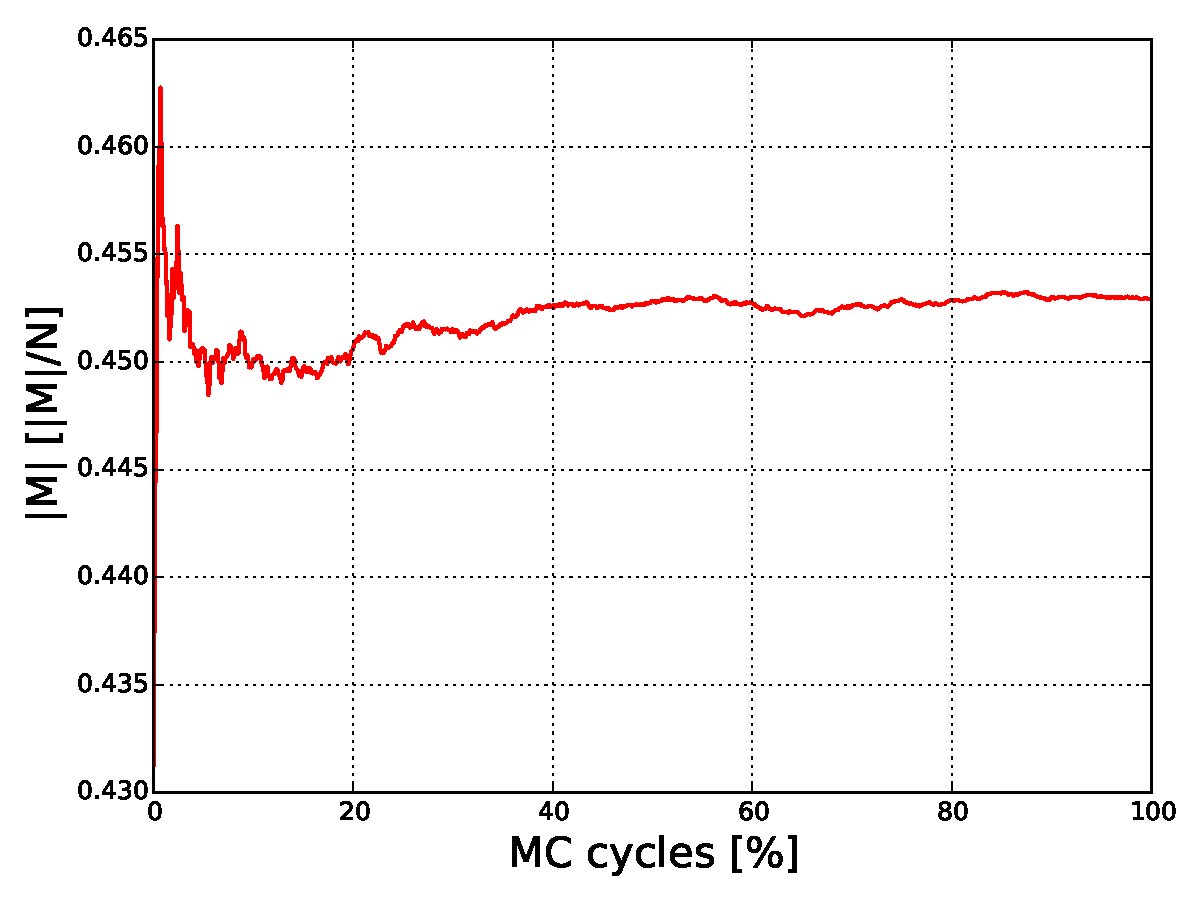
\includegraphics[width=\linewidth]{result/bilder/20x20/M-N20-T24}
        \caption{}
    \end{subfigure}%
    ~ 
    \begin{subfigure}{0.5\textwidth}
        \centering
        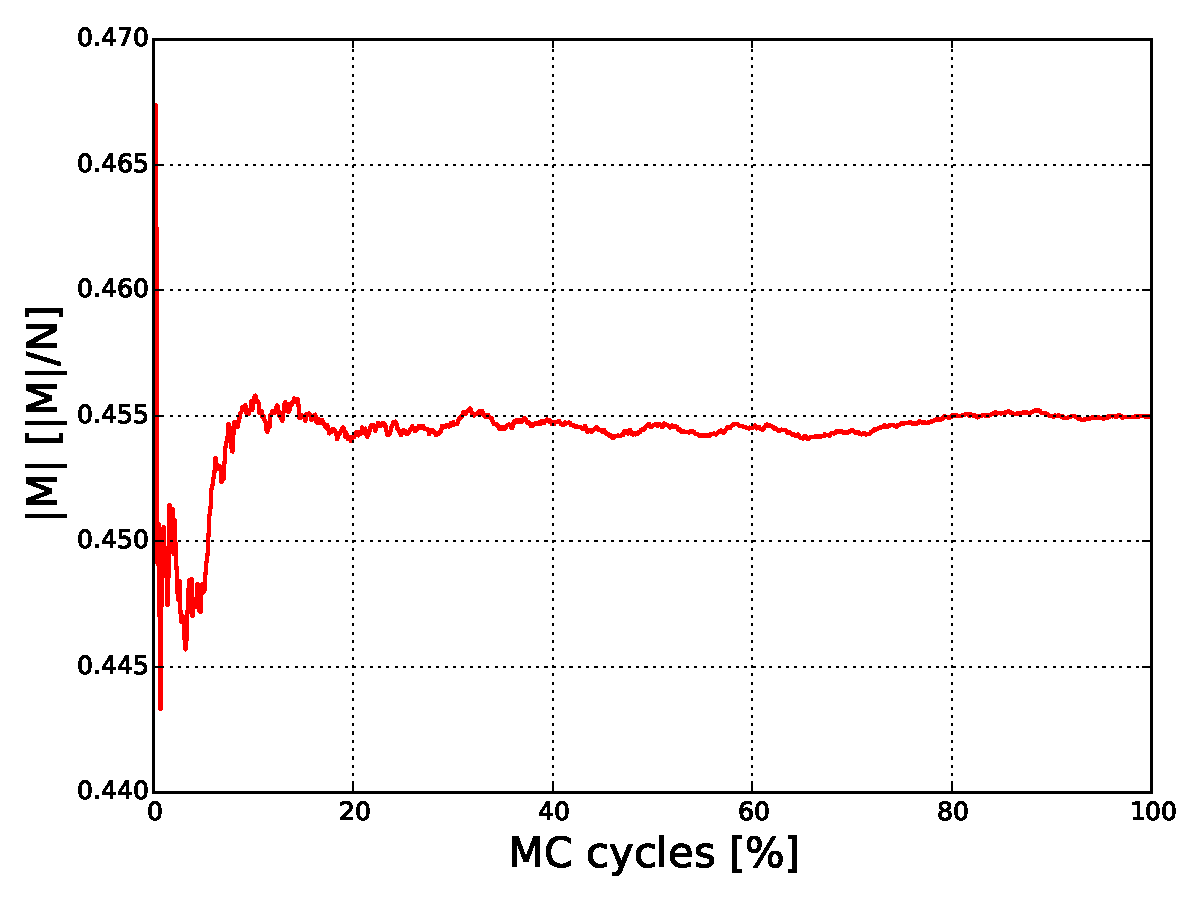
\includegraphics[width=\linewidth]{result/bilder/20x20/M-N20-T24-RNG}
        \caption{}
    \end{subfigure}
    \caption{The figure shows the development of |M| when T = 2.4. }
    \label{fig:}
\end{figure}


\begin{figure}[H]
    \centering
    \begin{subfigure}{0.5\textwidth}
        \centering
        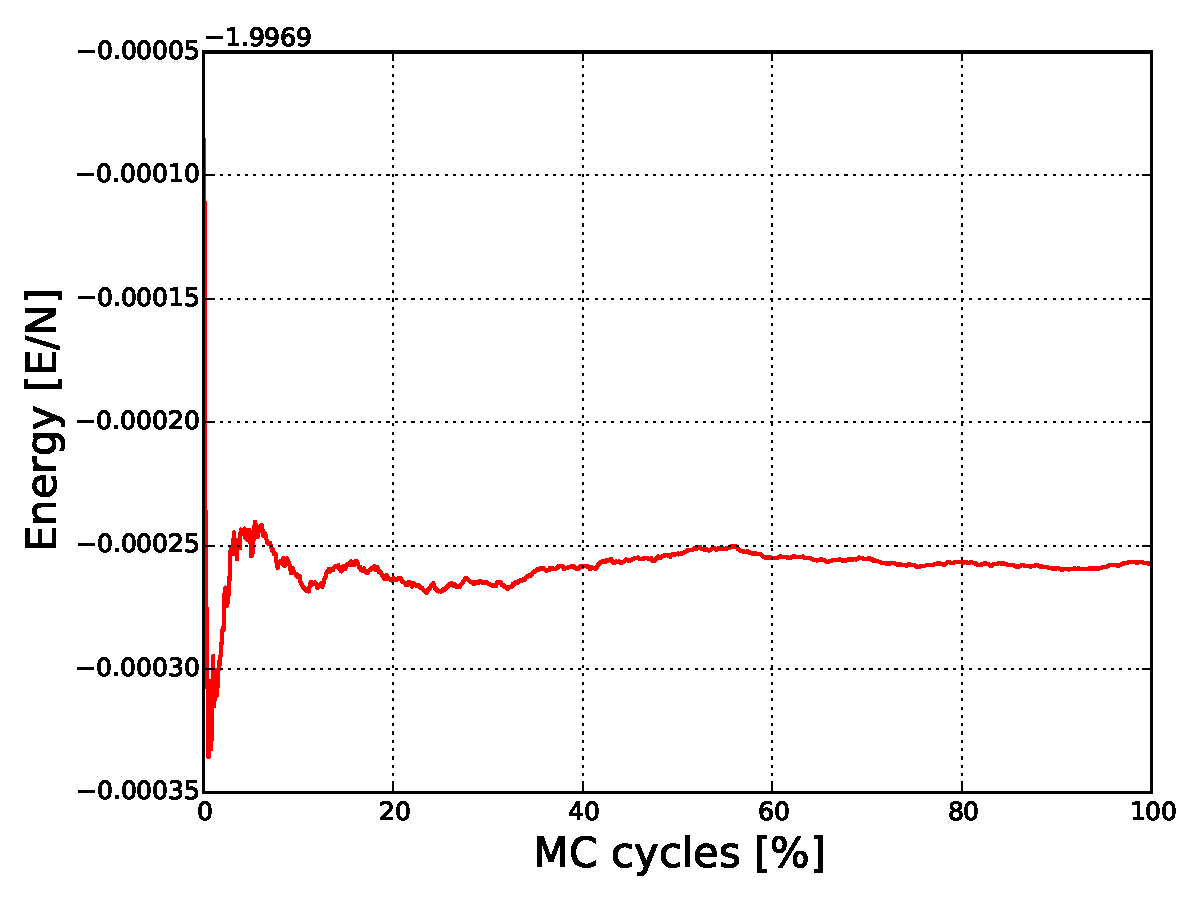
\includegraphics[width=\linewidth]{result/bilder/20x20/E-N20-T1-Term}
        \caption{}
    \end{subfigure}%
    ~ 
    \begin{subfigure}{0.5\textwidth}
        \centering
        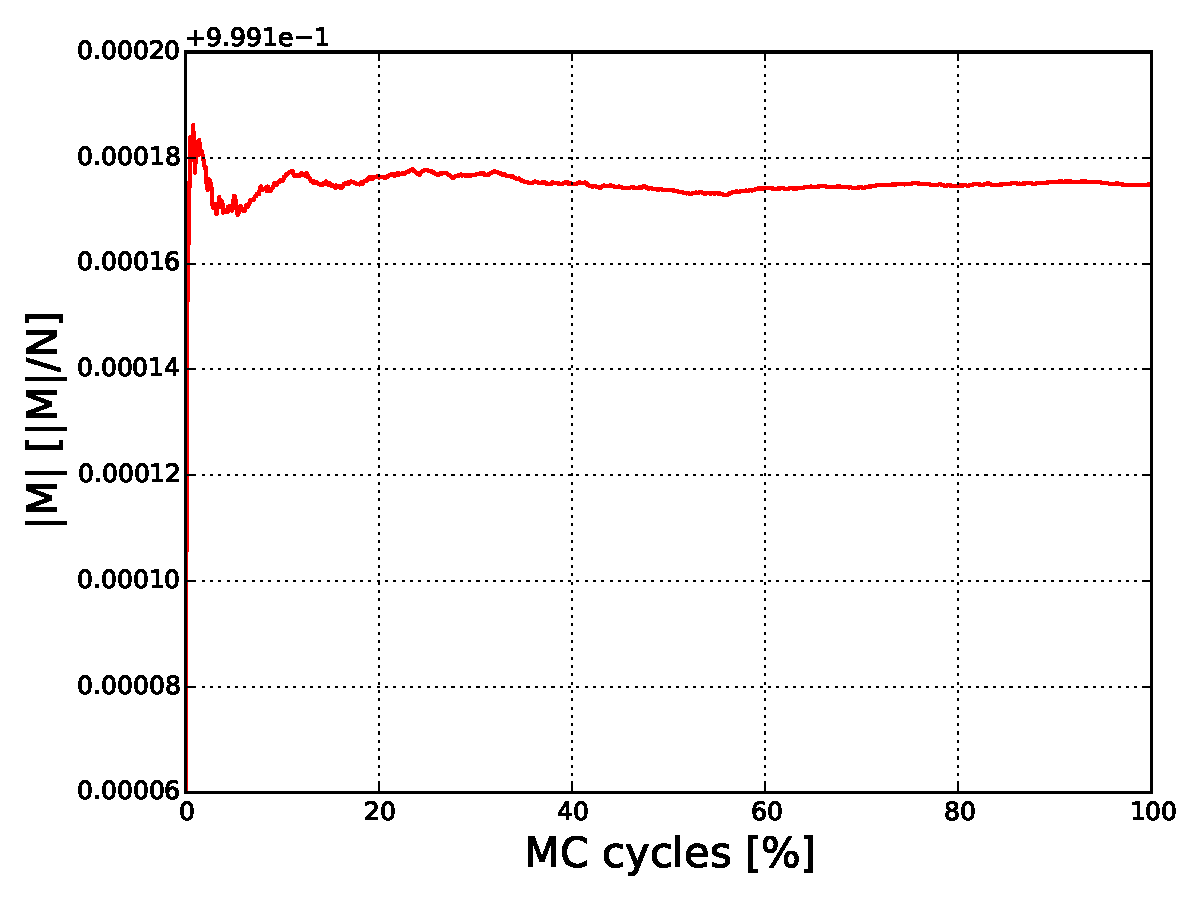
\includegraphics[width=\linewidth]{result/bilder/20x20/M-N20-T1-Term}
        \caption{}
    \end{subfigure}
    \caption{The figure shows the development of E when T = 1 when we dont use the first $10^5$ steps.  }
    \label{fig:equilibrium}
\end{figure}

For most of the figures in this section, almost 40\% of the MC seem to be used for obtaining equilibrium, but when removing one hundred thousand Monte Carlo cycles equilibrium seem to be obtained almost immediately. The first results are so bad that the system uses a longer time to achieve equilibrium, because the system needs to compensate for the first results. When removing this first part all the results that are used to calculate the expectation value is of good quality. For the rest of the report $10^5$ Monte Carlo cycles will be used to obtain equilibrium. If you have a lot of computational power and time, one can use use $10^6$ to obtain equilibrium. 



















\pagebreak
\subsection{Accepted configurations}

In this section acceptance of configurations for a 20x20 grid is studied. All grids were simulated for one million Monte Carlo cycles. Unless something else is specified in the figure, the left figure is for a initial configuration of the spin in the same direction and the right figure is for a random configuration. 

\begin{figure}[H]
    \centering
    \begin{subfigure}{0.5\textwidth}
        \centering
        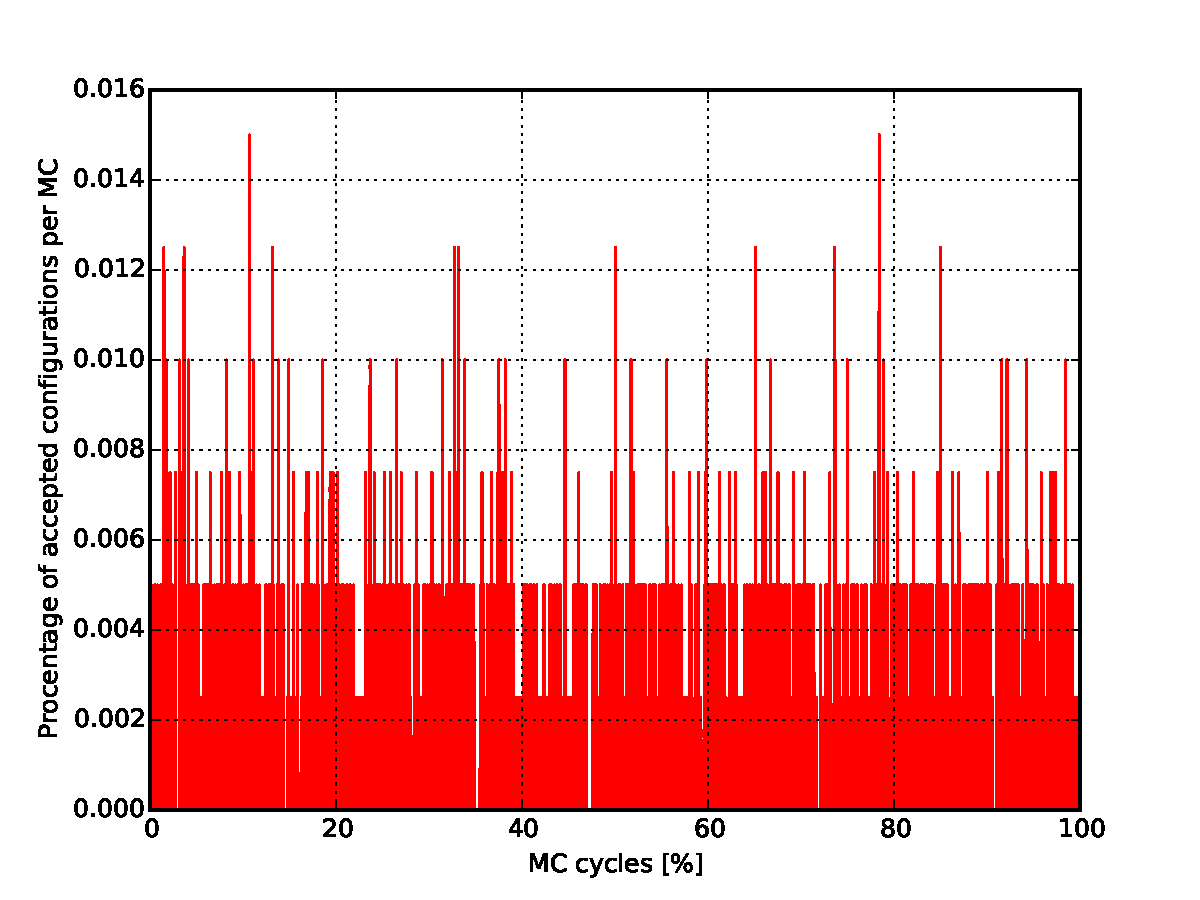
\includegraphics[width=\linewidth]{result/bilder/config/energy22-MC1000000T1-configN20}
        \caption{}
    \end{subfigure}%
    ~ 
    \begin{subfigure}{0.5\textwidth}
        \centering
        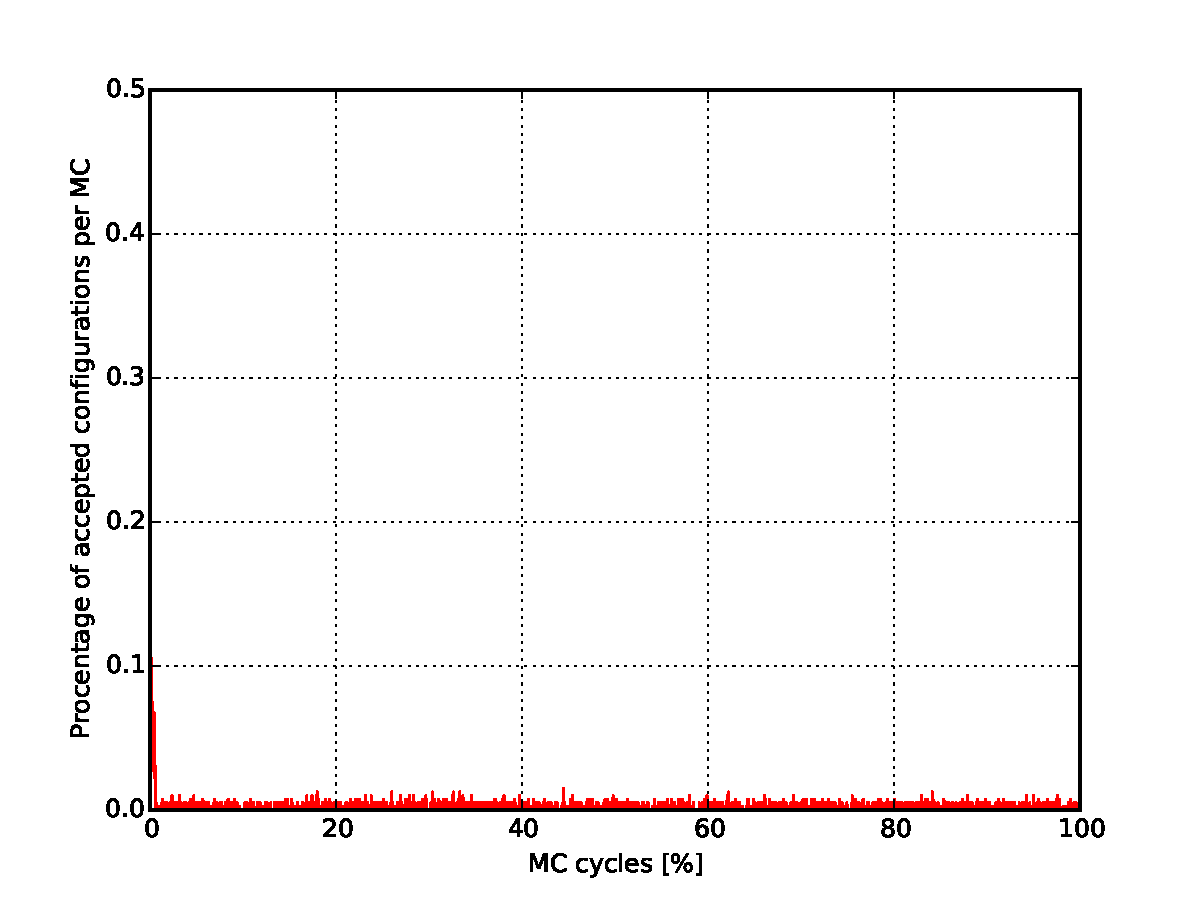
\includegraphics[width=\linewidth]{result/bilder/config/energy22-MC1000000T1-config-RNGN20}
        \caption{}
    \end{subfigure}
    \caption{This figure shows how the acceptance of configurations develop over time. T = 1 and for N=$10^6$. }
    \label{fig:config-T1}
\end{figure}

\begin{figure}[H]
    \centering
    \begin{subfigure}{0.5\textwidth}
        \centering
        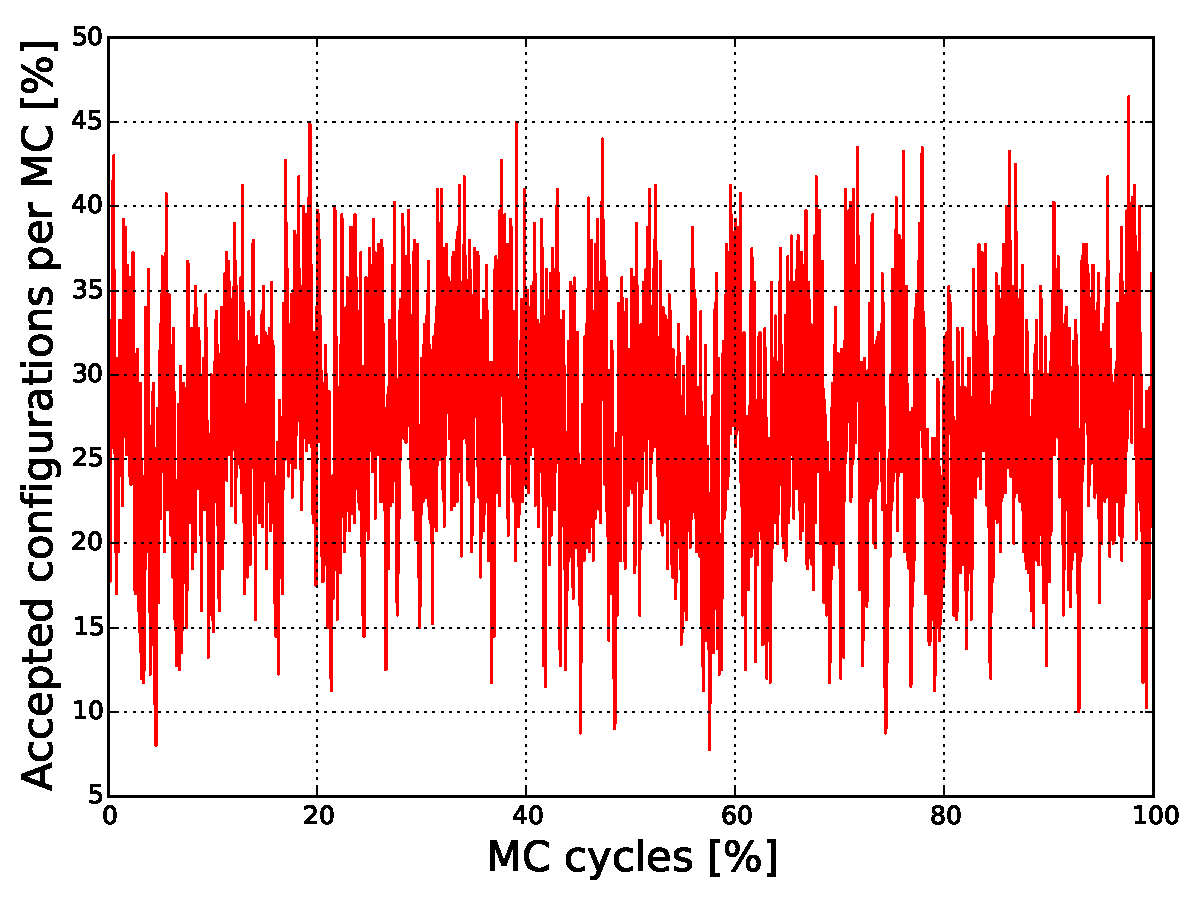
\includegraphics[width=\linewidth]{result/bilder/config/energy22-MC1000000T24-configN20}
        \caption{}
    \end{subfigure}%
    ~ 
    \begin{subfigure}{0.5\textwidth}
        \centering
        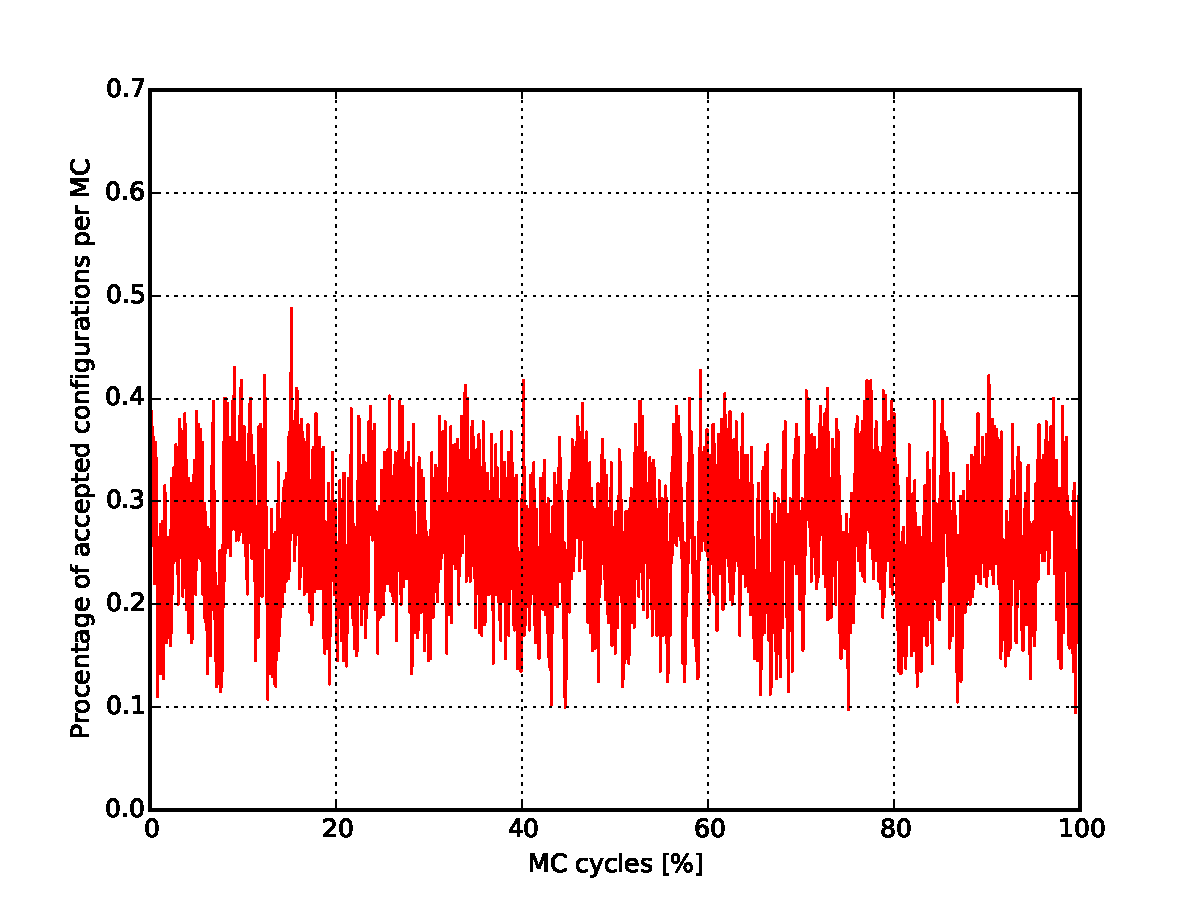
\includegraphics[width=\linewidth]{result/bilder/config/energy22-MC1000000T24-config-RNGN20}
        \caption{}
    \end{subfigure}
    \caption{This figure shows how the acceptance of configurations develop over time. T = 2.4 and for N=$10^6$. }
    \label{fig:config-T24}
\end{figure}

There are two things worth noting. First the difference between is non-existent and second there is a huge increase in percentage of accepted configurations when we increase the temperature. This is because of the energy difference acceptance that was discussed in section \ref{sec:metro}. When we go higher in temperature, the probability for accepting a state becomes larger.

















\pagebreak
\subsection{Probability distribution}

\todo{This is not done}

\begin{figure}[H]
    \centering
    \begin{subfigure}{0.5\textwidth}
        \centering
        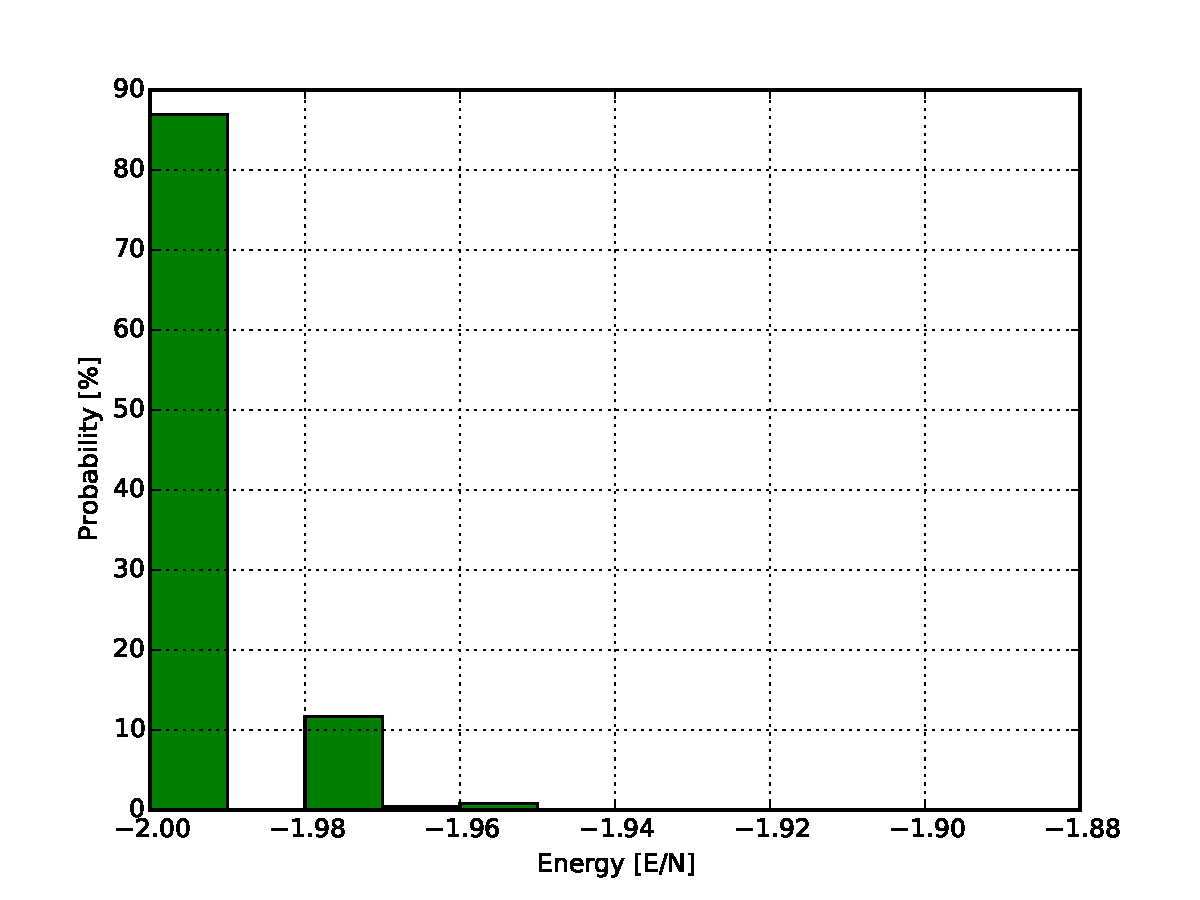
\includegraphics[width=\linewidth]{result/bilder/hist/MC1000000T1-distN20-hist}
        \caption{}
    \end{subfigure}%
    ~ 
    \begin{subfigure}{0.5\textwidth}
        \centering
        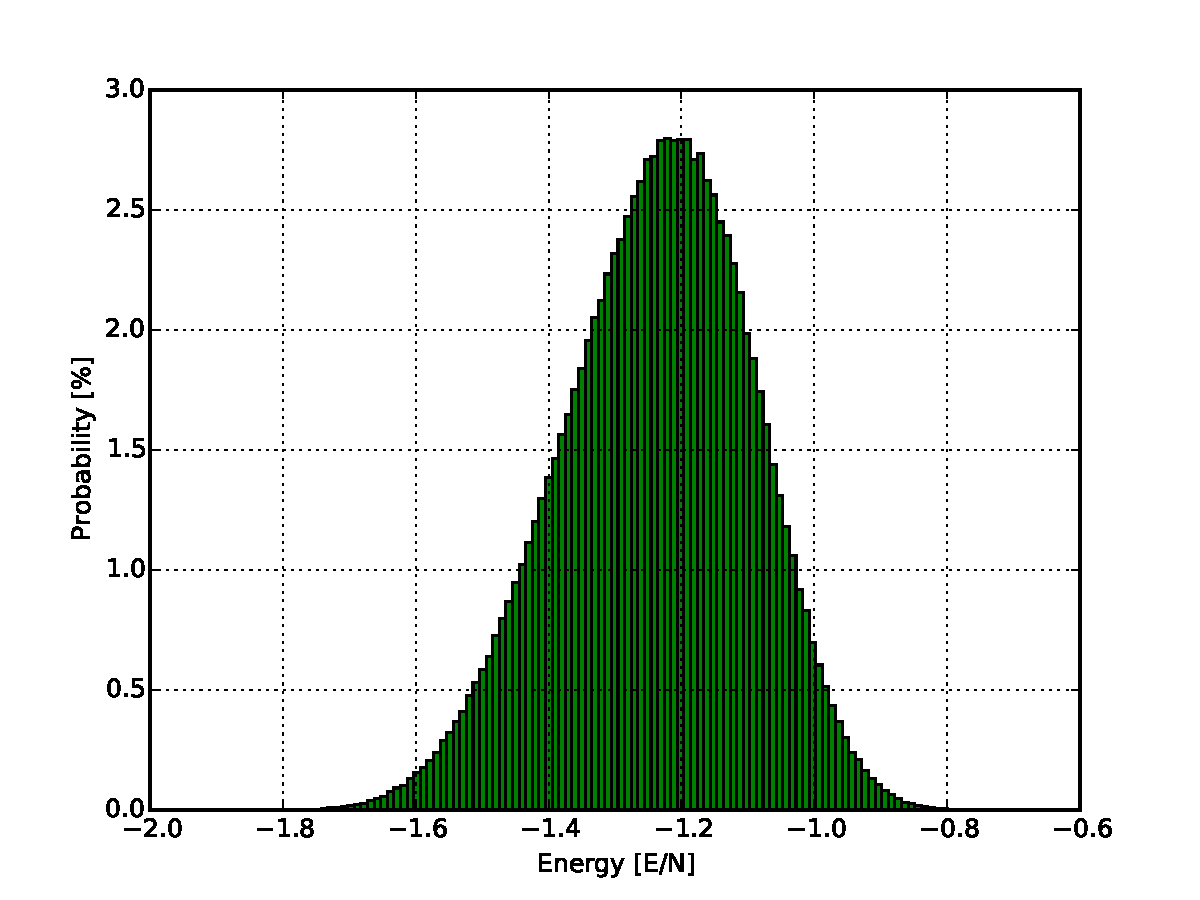
\includegraphics[width=\linewidth]{result/bilder/hist/MC1000000T24-distN20-hist}
        \caption{}
    \end{subfigure}
    \caption{a) }
    \label{fig:tc-chi-cv}
\end{figure}























\pagebreak
\subsection{Phase transition}



\subsubsection{Numerical studies of phase transition}

Several simulations were made with different L. Below a selected few of these simulations are shown. All the data and figures for this section are available at my \href{https://github.com/erikfsk/Project-4/tree/master/Project4/Result/4e/}{\textcolor{blue}{github}}. The figures below were created with a python \href{https://github.com/erikfsk/Project-4/blob/master/Project4/Result/4e/plot-4e.py}{\color{blue}{script}}.

\begin{figure}[H]
    \centering
    \begin{subfigure}{0.5\textwidth}
        \centering
        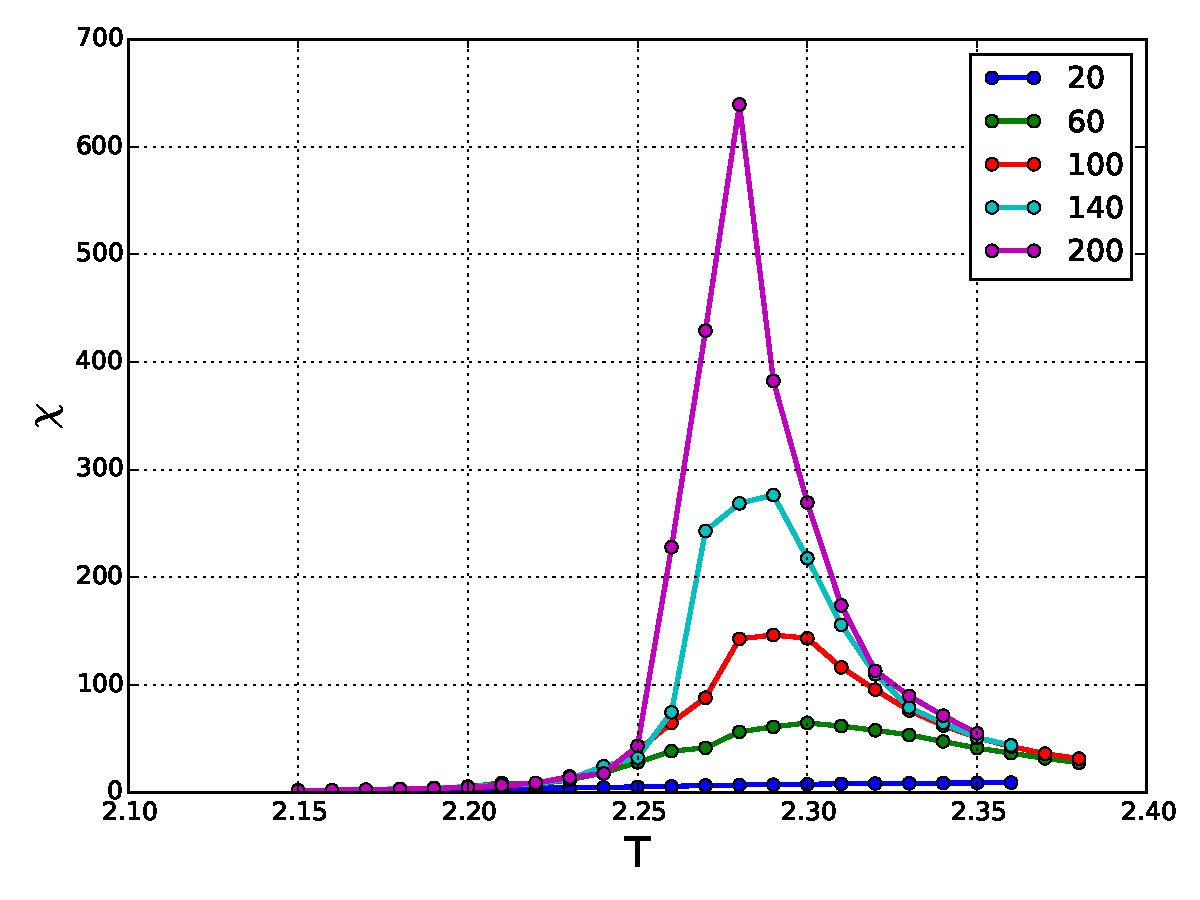
\includegraphics[width=\linewidth]{result/bilder/Tc/chi-Tc}
        \caption{}
    \end{subfigure}%
    ~ 
    \begin{subfigure}{0.5\textwidth}
        \centering
        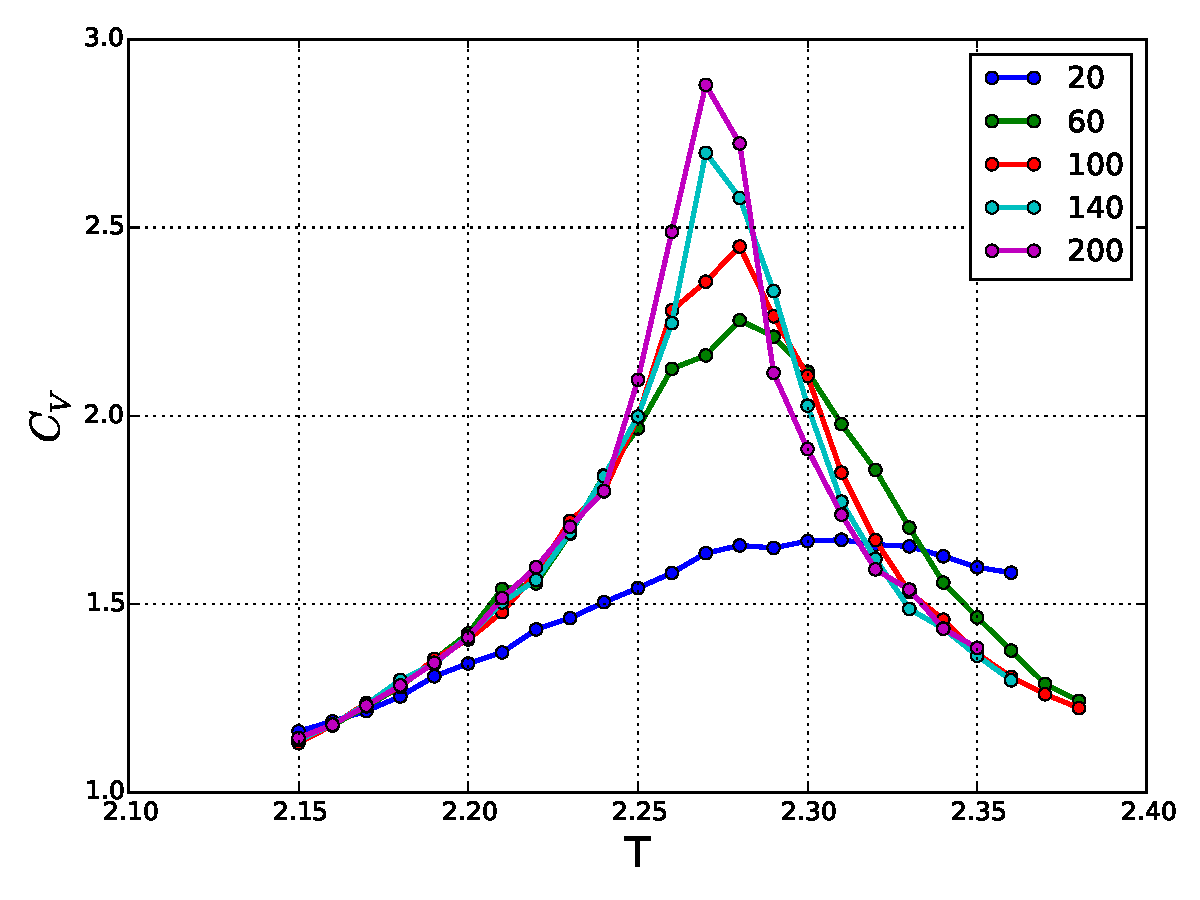
\includegraphics[width=\linewidth]{result/bilder/Tc/cv-Tc}
        \caption{}
    \end{subfigure}
    \caption{a) }
    \label{fig:tc-chi-cv}
\end{figure}

\begin{figure}[H]
    \centering
    \begin{subfigure}{0.5\textwidth}
        \centering
        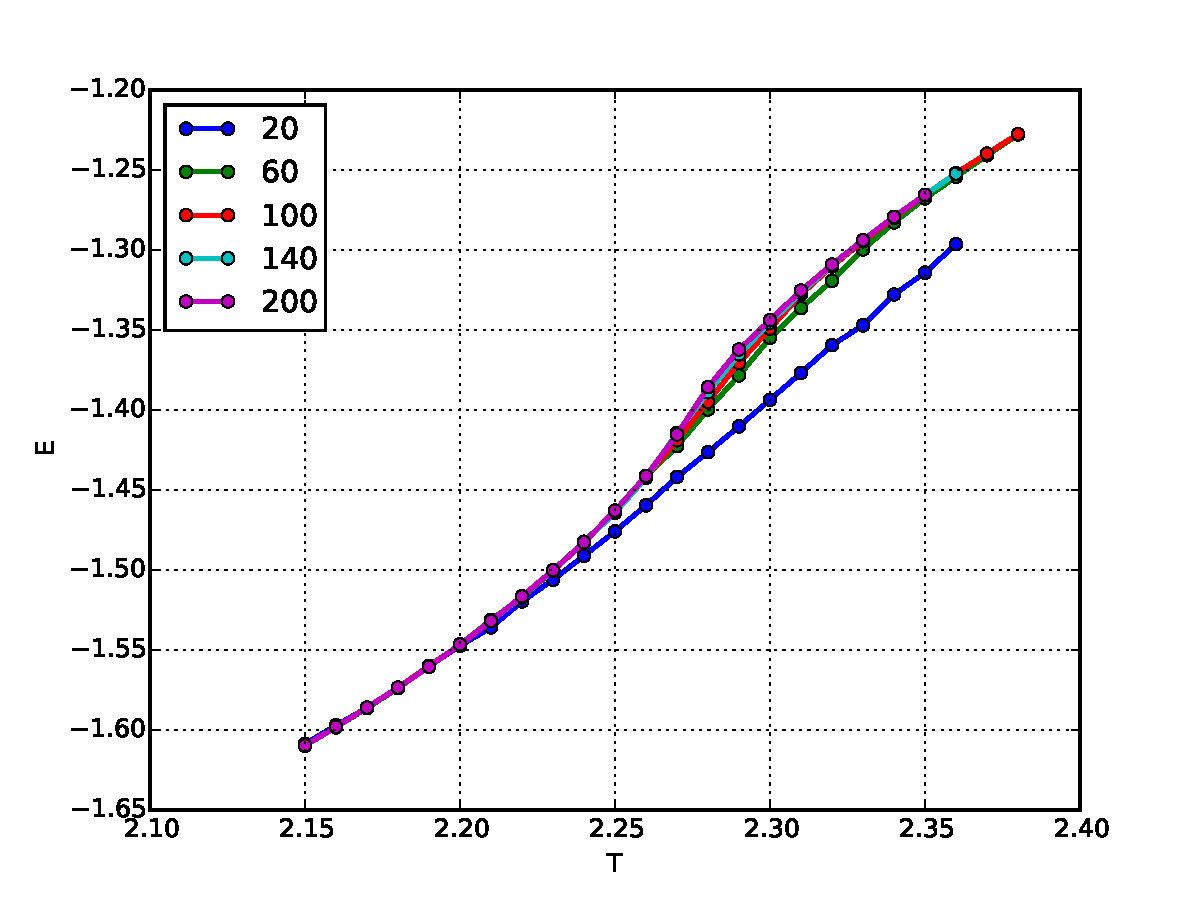
\includegraphics[width=\linewidth]{result/bilder/Tc/e-Tc}
        \caption{}
    \end{subfigure}%
    ~ 
    \begin{subfigure}{0.5\textwidth}
        \centering
        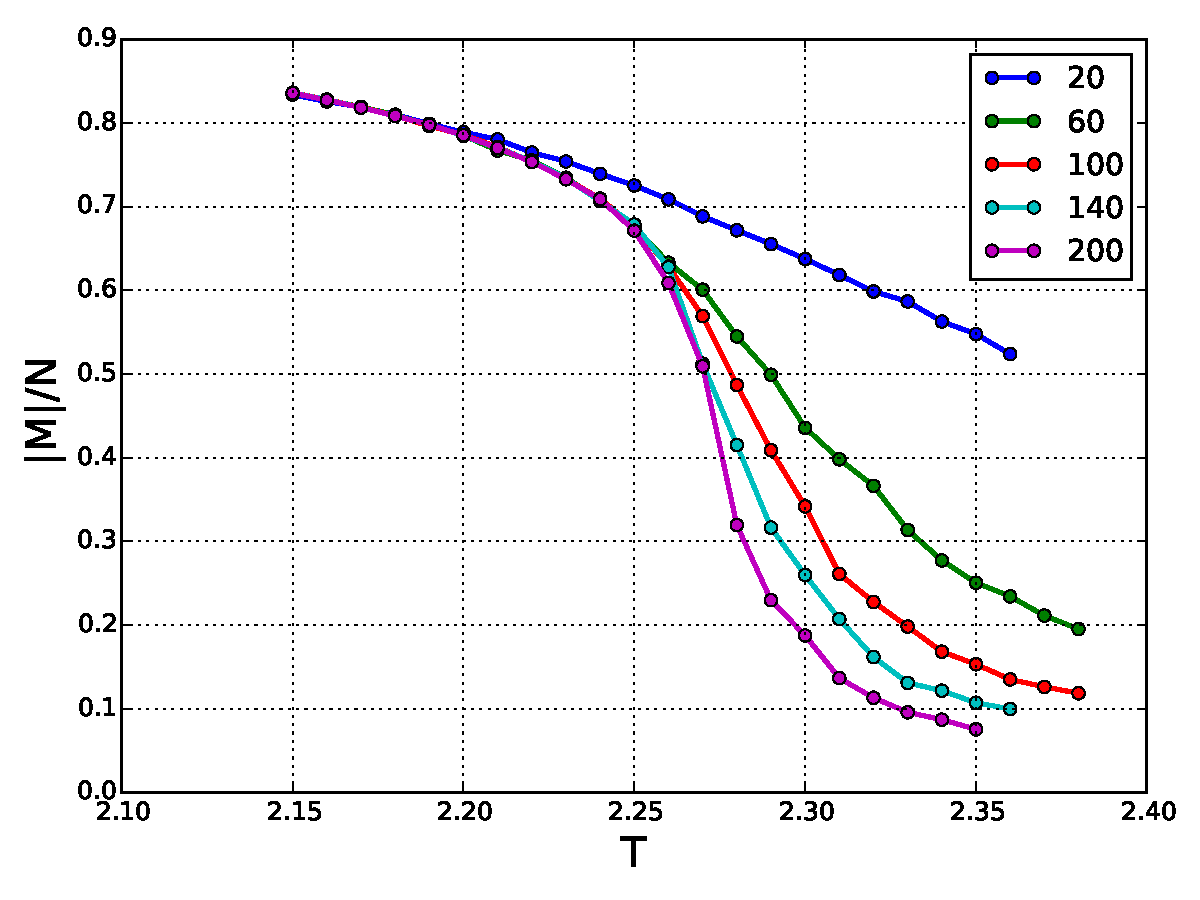
\includegraphics[width=\linewidth]{result/bilder/Tc/m-Tc}
        \caption{}
    \end{subfigure}
    \caption{a) }
    \label{fig:tc-E-M}
\end{figure}












\pagebreak
\subsubsection{Extracting the critical temperature}


% \begin{align*}
%     &T_C (L) - T_C (L=\infty) = a L^{\frac{-1}{v}}
% \end{align*}

% \begin{align*}
%     &T_C (L_i) - T_C (L_j) = a 
%     \left(
%     L_i^{\frac{-1}{v}}-L_j^{\frac{-1}{v}}
%     \right)
%     \\
%     &a = 
%     \frac{T_C (L_i) - T_C (L_j)} 
%     {
%     L_i^{\frac{-1}{v}}-L_j^{\frac{-1}{v}}
%     }
% \end{align*}

To extract a equation \ref{eq:find-a} is used. The result can be seen in table \ref{tab:extracting a}.

\begin{center}
\label{tab:extracting a}
\captionof{table}{The table shows how a differ for which $L_i$ and $L_j$ one uses. The values for $T_C$ were picked from figure \ref{fig:tc-chi-cv} a)}
\begin{tabularx}{\textwidth}{c X c X c X c X c}
    \hline 
    \hline 
        $L_i$ && $L_j$ && $T_{C_i}$ && $T_{C_j}$ && a\\ 
    \hline
        60      &&      100     &&  2.30  &&  2.29  && 0.00025 \\
        60      &&      140     &&  2.30  &&  2.28  && 0.00025 \\
        60      &&      200     &&  2.30  &&  2.27  && 0.0002142 \\
        100     &&      140     &&  2.29  &&  2.28  && 0.00025 \\
        100     &&      200     &&  2.29  &&  2.27  && 0.0002 \\
        140     &&      200     &&  2.28  &&  2.27  && 0.0001666 \\
    \hline
\end{tabularx}
\end{center}

From the values for a above, we can extract the average value of a, $\overline{a}$.
 $\overline{a}$ is 0.0002218. $\overline{a}$ is used in equation \ref{eq:t-c}. The results are in table \ref{tab:t-c}.

\begin{center}
\label{tab:t-c}
\captionof{table}{The table shows how a differ for which $L_i$ and $L_j$ one uses. The values for $T_C$ were picked from figure \ref{fig:tc-chi-cv} a)}
\begin{tabularx}{\textwidth}{c X c X c X c }
    \hline 
    \hline 
        $L_i$ && $T_C(L_i)$ && $T_C(\infty)$ with $\overline{a}$ \\ 
    \hline
        60      &&  2.30  && 2.2999\\
        100     &&  2.29  && 2.2899\\
        140     &&  2.28  && 2.2799\\
        200     &&  2.27  && 2.2699\\
    \hline
\end{tabularx}
\end{center}

An other way to calculate the critical temperature for an infinite lattice is to plot the finite $T_C$ versus the 1/L. And then make a polynomial fit of first degree. The intersection with the y-axis is the critical temperature for a infinite lattice.

\begin{figure}[H]
    \centering
    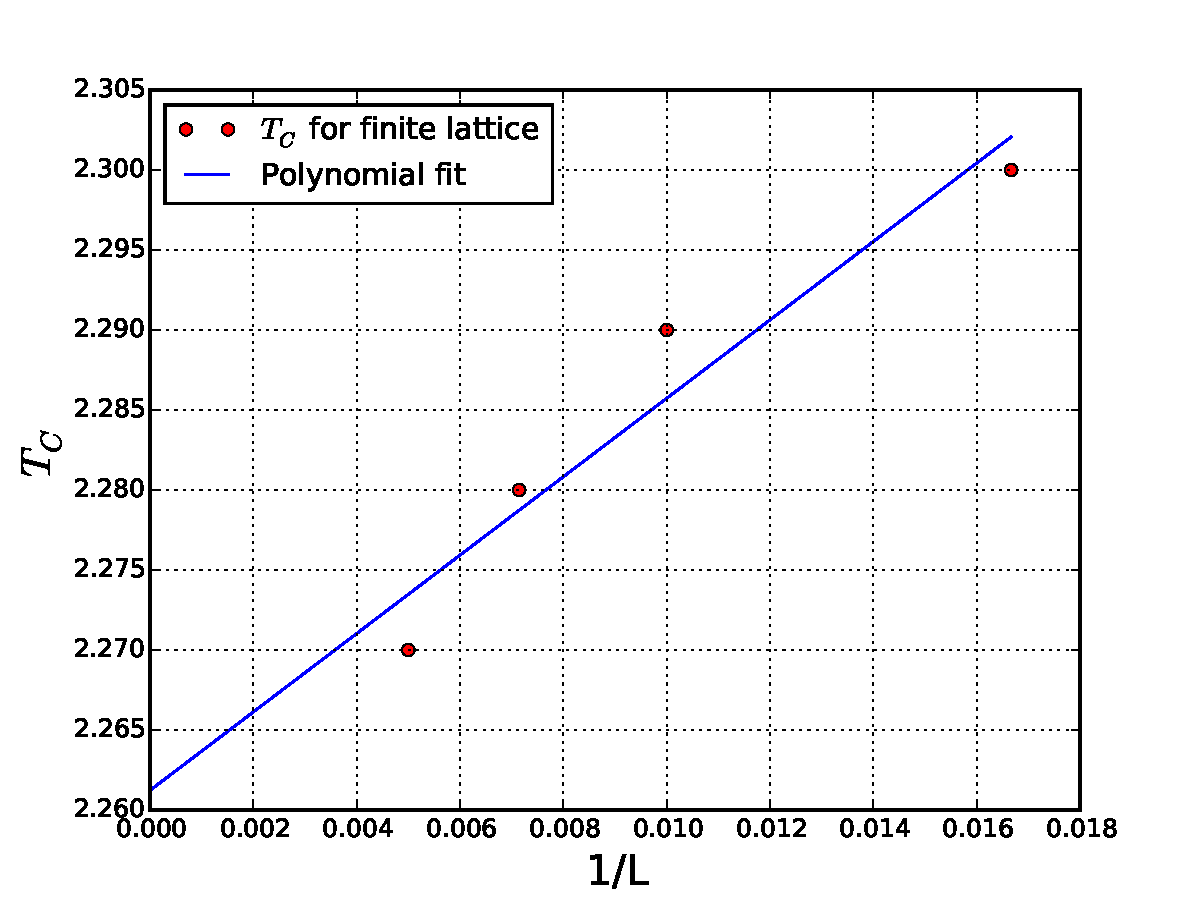
\includegraphics[width=0.5\linewidth]{result/bilder/tc/polyfit}
    \caption{This figure shows the linear regression of the $T_C$ from the finite lattices. From the graph one can read out the y-axis intersection, 2.261}
    \label{fig:polyfit}
\end{figure}

